\documentclass{article} % For LaTeX2e
\usepackage{nips14submit_e,times}
\usepackage{hyperref}
\usepackage{url}
\usepackage{amssymb,amsmath,amsthm}
\usepackage{subfigure}
\usepackage{tikz}
\usepackage{graphicx}
\usepackage{enumitem}
\usepackage{multirow}
\usepackage{algorithm,algorithmic}
\usetikzlibrary{positioning,decorations.pathreplacing}


% abbreviations
\def\eg{\emph{e.g.}}
\def\Eg{\emph{E.g.}}
\def\etal{\emph{et al.}}

% names - lowercase
\newcommand{\fracnet}{FractalNet}
\newcommand{\fracnets}{FractalNets}
\newcommand{\resnet}{ResNet}
\newcommand{\resnets}{ResNets}
\newcommand{\dropout}{dropout}
\newcommand{\dropconn}{drop-connect}
\newcommand{\droppath}{drop-path}

% names - uppercase
\newcommand{\Fracnet}{FractalNet}
\newcommand{\Fracnets}{FractalNets}
\newcommand{\Resnet}{ResNet}
\newcommand{\Resnets}{ResNets}
\newcommand{\Dropout}{Dropout}
\newcommand{\Dropconn}{Drop-connect}
\newcommand{\Droppath}{Drop-path}


\title{Convolutional Kernel Networks}

\author{
   Julien Mairal, Piotr Koniusz, Zaid Harchaoui, and Cordelia Schmid \\
   Inria\thanks{LEAR team, Inria Grenoble, Laboratoire Jean Kuntzmann, CNRS, Univ. Grenoble Alpes, France.} \\
   \texttt{firstname.lastname@inria.fr}
}

% The \author macro works with any number of authors. There are two commands
% used to separate the names and addresses of multiple authors: \And and \AND.
%
% Using \And between authors leaves it to \LaTeX{} to determine where to break
% the lines. Using \AND forces a linebreak at that point. So, if \LaTeX{}
% puts 3 of 4 authors names on the first line, and the last on the second
% line, try using \AND instead of \And before the third author name.

\newcommand{\fix}{\marginpar{FIX}}
\newcommand{\new}{\marginpar{NEW}}

\nipsfinalcopy % Uncomment for camera-ready version

\begin{document}


\maketitle

\begin{abstract}
   \begin{abstract}

We propose a convolutional neural network (CNN) architecture for facial expression recognition. The proposed architecture is independent of any hand-crafted feature extraction and performs better than the earlier proposed convolutional neural network based approaches. We visualize the automatically extracted features which have been learned by the network in order to provide a better understanding. The standard datasets, i.e. Extended Cohn-Kanade (CKP) and MMI Facial Expression Databse are used for the quantitative evaluation. On the CKP set the current state of the art approach, using CNNs, achieves an accuracy of 99.2\%. For the MMI dataset, currently the best accuracy for emotion recognition is 93.33\%. The proposed architecture achieves $99.6$\% for CKP and $98.63$\% for MMI, therefore performing better than the state of the art using CNNs. Automatic facial expression recognition has a broad spectrum of applications such as human-computer interaction and safety systems. This is due to the fact that non-verbal cues are important forms of communication and play a pivotal role in interpersonal communication. The performance of the proposed architecture endorses the efficacy and reliable usage of the proposed work for real world applications.

\end{abstract}
\end{abstract}

\section{Introduction}

%\cite{burger2001issues}
%\cite{fader2014open}
%\cite{voorhees1999trec}


%A huge leap forward in artificial intelligence will be achieved when
%machines will be able to answer any question expressed in natural
%language. As such, q

Question answering (QA) has been a long standing research problem in
natural language processing, with the first systems attempting to
answer questions by directly reading
documents \citep{voorhees2000building}. The development of large-scale Knowledge Bases (KBs) such as Freebase  \citep{bollacker2008freebase}
helped organize information into structured forms, prompting recent progress to focus on answering questions by converting them into logical forms that can be used to query such databases \citep{berant2013semantic,kwiatkowski-EtAl:2013:EMNLP,fader2014open}.

Unfortunately, KBs have intrinsic limitations such as their inevitable incompleteness and fixed schemas that cannot support all varieties of answers.
%
Since information extraction (IE) \citep{craven2000learning}, intended to
fill in missing information in KBs, is neither accurate nor
reliable enough, collections of raw textual resources and
documents such as Wikipedia will always contain more information.
%than KBs.
%
As a result, even if KBs can be satisfactory for closed-domain problems, they are unlikely
to scale up to answer general questions on any
topic.
%
Starting from this observation,
%here we propose  to study the problem
in this work we study the problem
of answering by directly reading documents.


Retrieving answers directly from text is harder than
from KBs because information is far less structured, is
indirectly and ambiguously expressed, and is usually scattered across multiple documents.
%
%This explains why, when a satisfactory KB is
%available -- which is typically only the case in closed domains --
%using it instead of raw text is preferred. %, because performance is better.
%
This explains why using a satisfactory KB---typically only available in closed domains---is preferred over raw text.
%
We postulate that before trying to provide answers that are not in
KBs, document-based QA systems should first reach KB-based systems'
performance in such closed domains, where clear comparison and
evaluation is possible.
%
To this end, this paper introduces {\sc WikiMovies}, a new
analysis tool that allows for measuring the performance of %loss induced on
QA systems when the knowledge source is switched from a KB to unstructured documents.
%
{\sc WikiMovies} contains $\sim$100k questions in the movie domain, and was designed
to be answerable by using either a perfect KB
(based on OMDb\footnote{\url{http://www.omdbapi.com}}), Wikipedia pages or an imperfect KB obtained through
running %a standard IE pipeline on those pages.
an engineered IE pipeline on those pages.

To bridge the gap between using a KB and reading documents directly,
we still lack appropriate machine learning algorithms. In this
work we propose the Key-Value Memory Network (KV-MemNN), a new neural network
architecture that generalizes the original Memory Network
\citep{sukhbaatar2015end} and can work with either knowledge source.
%
The KV-MemNN performs QA by first storing facts in a key-value
structured memory before reasoning on them in order to predict an
answer. The memory is designed so that the model learns to use keys to
address relevant memories with respect to the question, whose corresponding values are subsequently returned.
%
This structure allows the model to encode prior knowledge for the considered task
and to leverage possibly complex transforms between keys and values,
while still being trained using standard backpropagation via
stochastic gradient descent.

Our experiments on {\sc WikiMovies} indicate that, thanks to its key-value memory,
the KV-MemNN consistently outperforms the
original Memory Network, and reduces the gap between answering from a human-annotated KB,
from an automatically extracted KB or from directly reading Wikipedia.
%
We confirm our findings on  {\sc WikiQA} \citep{yang2015wikiqa},
another Wikipedia-based QA benchmark where no KB is available,
where we demonstrate that KV-MemNN can reach state-of-the-art results---surpassing
the most recent attention-based neural network models.


\subsection{Related Work}\label{sec:related}
\section{Related work}\label{s:related}

\begin{figure}[t]
\centering
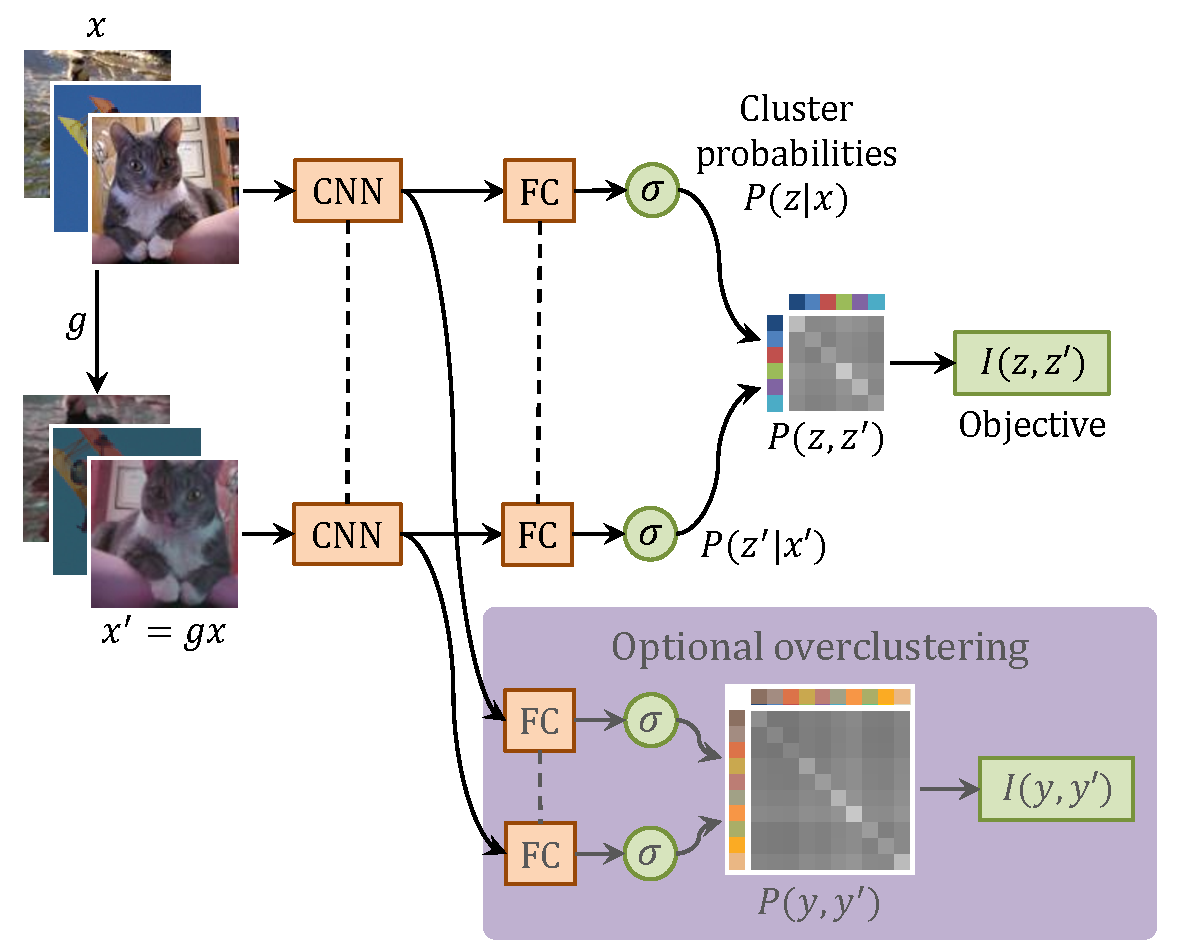
\includegraphics[width=0.95\columnwidth]{paper_imgs/overview1.pdf}
\caption{\label{f:overview}\methodnameshort for image clustering. Dashed line denotes shared parameters, $g$ is a random transformation, and $I$ denotes mutual information~(\cref{e:loss_expanded}).}
\end{figure}


\begin{figure*}
%\captionsetup{justification=centering}
\setlength\tabcolsep{2.2pt} % default value: 6pt

\begin{tabular}{c c c c c c}
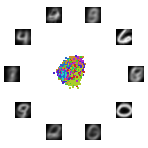
\includegraphics[height=0.16\textwidth]{experiments2_files/mnist_progression/726_run_1_colour_0_pointcloud_0.png} & 
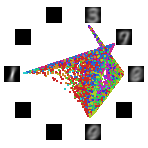
\includegraphics[height=0.16\textwidth]{experiments2_files/mnist_progression/726_run_1_colour_0_pointcloud_3.png} & 
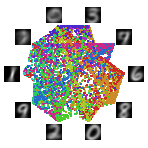
\includegraphics[height=0.16\textwidth]{experiments2_files/mnist_progression/726_run_1_colour_0_pointcloud_10.png} & 
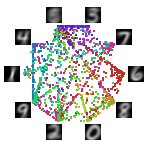
\includegraphics[height=0.16\textwidth]{experiments2_files/mnist_progression/726_run_1_colour_0_pointcloud_30.png} & 
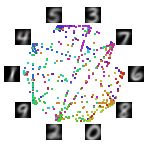
\includegraphics[height=0.16\textwidth]{experiments2_files/mnist_progression/726_run_1_colour_0_pointcloud_101.png} & 
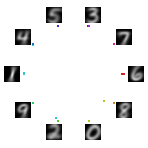
\includegraphics[height=0.16\textwidth]{experiments2_files/mnist_progression/726_run_1_colour_0_pointcloud_1000.png} 
\end{tabular}

\caption{\label{f:mnist_dots} Training with \methodnameshort on unlabelled MNIST in successive epochs from random initialisation (left). The network directly outputs cluster assignment probabilities for input images, and each is rendered as a coordinate by convex combination of 10 cluster vertices. There is no cherry-picking as the entire dataset is shown in every snapshot. Ground truth labelling (unseen by model) is given by colour. At each cluster the average image of its assignees is shown. With neither labels nor heuristics, the clusters discovered by \methodnameshort correspond perfectly to unique digits, with one-hot certain prediction (right).}
\end{figure*}


\paragraph{Co-clustering and mutual information.}

The use of information as a criterion to learn representations is not new. One of the earliest works to do so is by Becker and Hinton~\cite{becker1992self}.
More generally, learning from paired data has been explored in co-clustering~\cite{hartigan1972direct, dhillon2003information} and in other works~\cite{wang2010information} that build on the information bottleneck principle~\cite{friedman2001multivariate}.

Several recent papers have used information as a tool to train deep networks in particular.
IMSAT~\cite{hu2017learning} maximises mutual information between data and its representation and DeepINFOMAX~\cite{hjelm2018learning} maximizes information between spatially-preserved features and compact features.
However, IMSAT and DeepINFOMAX combine information with other criteria, whereas in our method information is the only criterion used.
Furthermore, both IMSAT and DeepINFOMAX compute mutual information over continuous random variables, which requires complex estimators~\cite{belghazi2018mine}, whereas \methodnameshort does so for discrete variables with simple and exact computations.
Finally, DeepINFOMAX considers the information $I(\bx, f(\bx))$ between the features $\bx$ and a deterministic function $f(\bx)$ of it, which is in principle the same as the entropy $H(\bx)$; in contrast, in \methodnameshort information does not trivially reduce to  entropy.

\paragraph{Semantic clustering versus intermediate representation learning.}
In semantic clustering, the learned function directly outputs discrete assignments for high level (i.e. semantic) clusters. Intermediate representation learners, on the other hand, produce continuous, distributed, high-dimensional representations that must be post-processed, for example by k-means, to obtain the discrete low-cardinality assignments required for unsupervised semantic clustering. The latter includes objectives such as generative autoencoder image reconstruction~\cite{vincent2010stacked},  triplets~\cite{schultz2004learning} and spatial-temporal order or context prediction~\cite{lee2017unsupervised,cruz2017deeppermnet,doersch2015unsupervised}, for example predicting patch proximity~\cite{isola2015learning}, solving jigsaw puzzles~\cite{noroozi2016unsupervised} and inpainting~\cite{pathak2016context}. Note it also includes a number of clustering methods (DeepCluster~\cite{caron2018deep}, exemplars~\cite{dosovitskiy2015discriminative}) where the clustering is only auxiliary; a clustering-style objective is used but does not produce groups with semantic correspondence. For example, DeepCluster~\cite{caron2018deep} is a state-of-the-art method for learning highly-transferable intermediate features using overclustering as a proxy task, but does not automatically find semantically meaningful clusters. As these methods use auxiliary objectives divorced from the semantic clustering objective, it is unsurprising that they perform worse than \methodnameshort~(\cref{s:experiments}), which directly optimises for it, training the network end-to-end with the final clusterer implicitly wrapped inside.




\paragraph{Optimising image-to-image distance.}

Many approaches to deep clustering, whether semantic or auxiliary, utilise a distance function between input images that approximates a given grouping criterion.
Agglomerative clustering~\cite{bautista2016cliquecnn} and partially ordered sets~\cite{bautista2017deep} of HOG features~\cite{dalal2005histograms} have been used to group images, and exemplars~\cite{dosovitskiy2015discriminative} define a group as a set of random transformations applied to a single image. Note the latter does not scale easily, in particular to image segmentation where a single $200\times 200$ image would call for 40k classes. DAC~\cite{chang2017deep}, JULE~\cite{yang2016joint}, DeepCluster~\cite{caron2018deep}, ADC~\cite{haeusser2018associative} and DEC~\cite{xie2016unsupervised} rely on the inherent visual consistency and disentangling properties~\cite{greff2015binding} of CNNs to produce cluster assignments, which are processed and reinforced in each iteration. 
The latter three are based on k-means style mechanisms to refine feature centroids, which is prone to degenerate solutions~\cite{caron2018deep} and thus needs explicit prevention mechanisms such as pre-training, cluster-reassignment or feature cleaning via PCA and whitening~\cite{xie2016unsupervised, caron2018deep}.

\begin{comment}
DAC is the only unsupervised clustering algorithm out of these that eschews k-means and agglomerative clustering for a different but similar clustering scheme, based on feature inner-products rather than distances.
DAC forms clusters gradually, in a self-paced manner, thus alleviating but not eliminating the risk of incurring degenerate solutions.
Furthermore, the nature of the optimisation, which reinforces bootstrapped class labels, creates a strong dependency on initialisation.

For unsupervised feature learning in general, i.e.\ where the training objective is not clustering, a large number of works explore using proxy learning tasks. 
There are two major directions:  generative tasks such as autoencoder image reconstruction~\cite{vincent2010stacked}, and spatial-temporal order or context prediction~\cite{lee2017unsupervised,cruz2017deeppermnet,doersch2015unsupervised}. The latter includes predicting patch proximity~\cite{isola2015learning}, solving jigsaw puzzles~\cite{noroozi2016unsupervised} and inpainting~\cite{pathak2016context}. 
In many cases they benefit from principled formulations that protect against degeneracy.
However, unlike the aforementioned clustering methods, the features learned by these methods need to be post-processed, for example using k-means, to cluster the data. 

\end{comment}

\paragraph{Invariance as a training objective.}

Optimising for function outputs to be persistent through spatio-temporal or non-material distortion is an idea shared by \methodnameshort with several works, including exemplars~\cite{dosovitskiy2015discriminative}, IMSAT~\cite{hu2017learning}, proximity prediction~\cite{isola2015learning}, the denoising objective of Tagger~\cite{greff2016tagger}, temporal slowness constraints~\cite{zou2012deep}, and optimising for features to be invariant to local image transformations~\cite{sohn2012learning,hui2013direct}.
More broadly, the problem of modelling data transformation has received significant attention in deep learning, one example being the transforming autoencoder~\cite{hinton2011transforming}.


% \section{Related work}\label{s:related}

% \paragraph{Co-clustering and mutual information.}

% The idea of learning a data representation by seeking the common parts of related observations is not new. 
% An early work is Becker and Hinton~\cite{becker1992self}, which maximises agreement between representations of 2D images to learn depth, using an objective corresponding to maximising mutual information between the input and the average of the data representations. 
% Co-learning has also been explored in the context of clustering by co-clustering methods, dating back to the pioneering work of Hartigan~\cite{hartigan72direct}. 
% Many information-theoretic variant of such approaches have been proposed, as discussed by~\cite{wang10information}, which are generally related to the information bottleneck principle~(\cite{friedman2001multivariate}). 

% A few works have employed mutual information in the context of unsupervised deep learning. IMSAT~\cite{hu2017learning} maximises mutual information between input data and their predicted discrete representations whilst encouraging the representations of augmented data points to be close to those of the original data points. 
% DeepINFOMAX~\cite{hjelm2018learning} maximises mutual information between spatially preserved features and compact features. There are some major differences with \methodnameshort. 
% Firstly, mutual information is used as an aid in these methods, as it increases the statistical predictivity between two random variables. 
% This contrasts with our method, where mutual information constitutes the loss applied directly to cluster assignments, meaning it is used as a clustering objective. 
% Secondly, both IMSAT and DeepINFOMAX compute mutual information over continuous random variables, which calls for an integral and is not computationally tractable, so estimators~\cite{belghazi2018mine} are used. 
% Since \methodnameshort maximises mutual information between cluster assignments and the number of clusters is discrete, computation is exact and straightforward. 
% Finally, DeepINFOMAX employs mutual information between function inputs and outputs, i.e. $I(x, f(x))$, but the conditional entropy component of mutual information $H(f(x) | x)$ is 0 when $f$ is deterministic, making the maximisation less meaningful. 
% In contrast \methodnameshort maximises mutual information between cluster assignments of separate images, i.e. $I(z, z')$ where $z$ and $z'$ are not functions of one other, making $H(z | z')$ a non-zero quantity that contributes to the optimisation as it can be minimised.

% \paragraph{Optimising image-to-image distance for clustering.}
% Many works for on unsupervised deep clustering involve establishing a scheme for estimating the semantic distance between input images, before training a function to learn this scheme. 
% CliqueCNN~\cite{bautista2016cliquecnn} trains a network to discriminate between cliques that are determined by applying agglomerative clustering on image features such as HOG~\cite{dalal2005histograms}. 
% In Exemplar CNNs~\cite{dosovitskiy2016discriminative}, each image and a its set of random transformations is considered a class, and a function is trained to discriminate between these surrogate classes. Like \methodnameshort, this method uses random transformations as a proxy for obtaining images with low semantic distance in the absence of label information. 
% Requiring one class per input image has a large memory footprint which makes Exemplar CNNs infeasible for segmentation (where patches are clustered instead of images, so a single 200x200 image would call for 40k classes). 

% \begin{figure}[t]
\centering
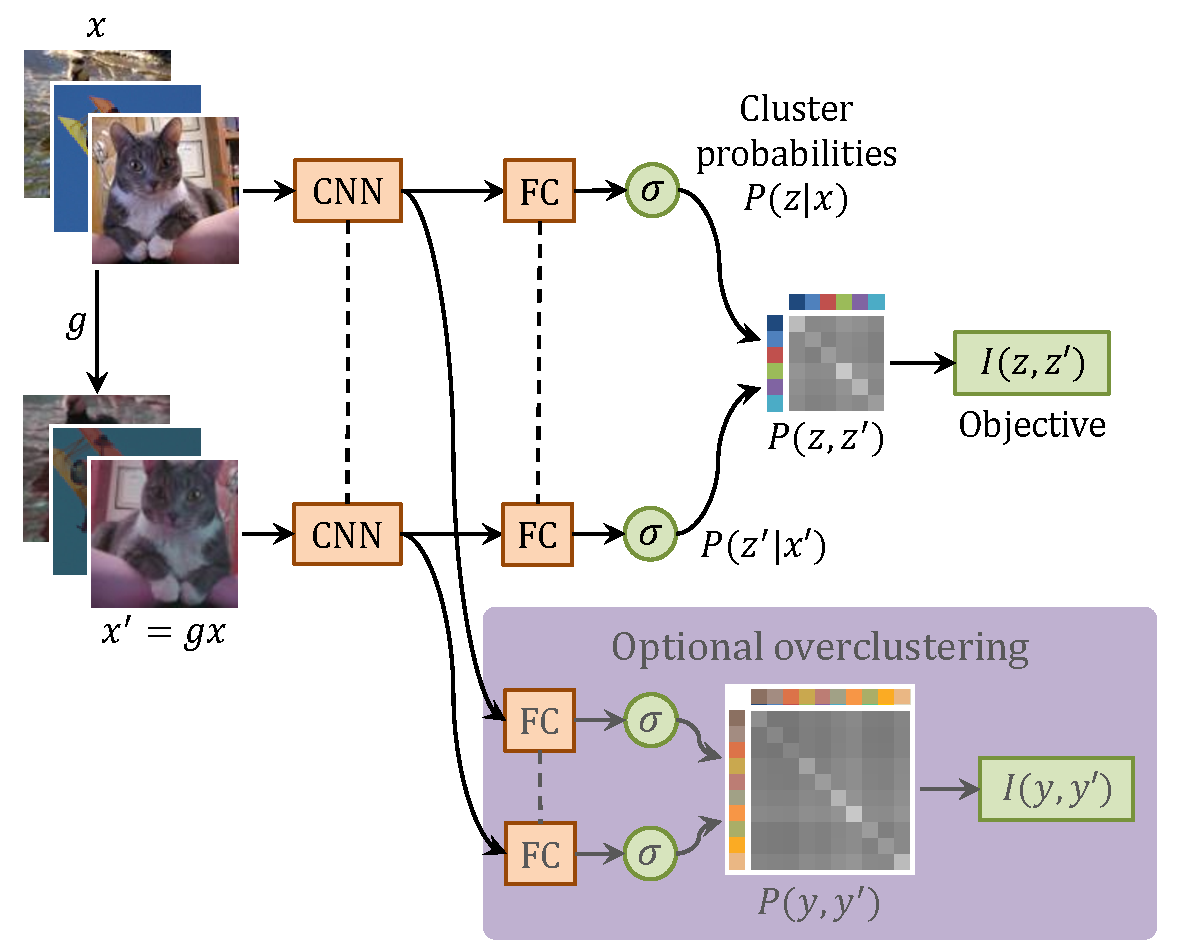
\includegraphics[width=0.95\columnwidth]{paper_imgs/overview1.pdf}
\caption{\label{f:overview}\methodnameshort for image clustering. Dashed line denotes shared parameters, $g$ is a random transformation, and $I$ denotes mutual information~(\cref{e:loss_expanded}).}
\end{figure}


% DAC~\cite{chang2017deep}, JULE~\cite{yang2016joint}, DeepCluster~\cite{caron2018deep}, Associative Deep Clustering~\cite{haeusser18associative} and DEC~\cite{xie2016unsupervised} all rely on the inherent visual consistency and disentangling properties~\cite{greff2015binding} of CNNs to produce meaningful cluster assignments, which are processed and reinforced in each iteration. 
% The latter three are based on using k-means to refine deep feature vectors, a mechanism which is prone to degenerate solutions~\cite{caron2018deep} and thus needs explicit prevention mechanisms such as pre-training, cluster-reassignment or feature cleaning via PCA and whitening ~\cite{xie2016unsupervised, caron2018deep}. 

% DAC is the only unsupervised clustering algorithm out of these that eschews k-means whilst training a network to directly produce cluster assignments, as \methodnameshort does. 
% A network is trained to produce cluster assignment probability distributions for each sample that are used as high level feature descriptors, and the dot product of different descriptors is treated as a proxy for inter-sample semantic distance (instead of Euclidian distance, which is used in the k-means based clusterers). 
% Training proceeds by maximising the dot product of close sample pairs, thus encouraging them to be assigned to the same cluster, whilst minimising the dot product for far pairs. 
% The nature of the optimisation means there is a strong dependency on initialisation and lack of protection against degenerate solutions such as clusters disappearing. 

% \paragraph{Proxy tasks for unsupervised feature learning.}
% For unsupervised feature learning in general, i.e. where the training objective is not clustering, a large number of works explore using proxy learning tasks. 
% There are two major camps:  generative tasks such as autoencoder image reconstruction~\cite{vincent2010stacked}, and spatial-temporal order or context prediction~\cite{lee2017unsupervised,cruz2017deeppermnet,doersch2015unsupervised}. The latter includes predicting patch proximity~\cite{isola2015learning}, solving jigsaw puzzles~(\cite{noroozi2016unsupervised}) and inpainting~(\cite{pathak2016context}). 
% In many cases they benefit from principled formulations that protect against degeneracy.
% However, unlike the aforementioned clustering methods, learned representations from these tasks constitute fine-grained continuous features rather than coarse cluster assignments, and thus must be post-processed, either by unsupervised clustering such as k-means or with label information via SVMs or fine-tuning, in order to produce semantic clusters.

% \paragraph{Invariance as a training objective.}
% Training for function outputs to be persistent through spatio-temporal distortion, noise distortion, or random transforms is an idea shared by \methodnameshort and several mentioned works, including Exemplar CNNs~\cite{dosovitskiy2016discriminative}, IMSAT~\cite{hu2017learning} and proximity prediction~\cite{isola2015learning}.
% It is also seen in Tagger~\cite{greff2016tagger}, which trains a function to denoise its input using several clusters to distribute the representation,~\cite{zou2012deep} which enforces a temporal slowness constraint on learned features, and~\cite{sohn2012learning,hui2013direct} which train for features invariant to local image transformations.




\section{Convolutional Multilayer Kernels}\label{sec:scattering}
The convolutional multilayer kernel is a generalization of the hierarchical kernel
descriptors introduced in computer vision~\cite{bo2011,bo2010}. The kernel produces a
sequence of image representations that are built on top of each other in a
multilayer fashion. Each layer can be interpreted as a non-linear
transformation of the previous one with additional spatial invariance. We call these
layers \emph{image feature maps}\footnote{In the kernel literature, ``feature map'' denotes the mapping between data points and their representation in a reproducing kernel Hilbert space (RKHS)~\cite{shawe2004}. Here, feature maps refer to spatial maps representing local image characteristics at everly location, as usual in the neural network literature~\cite{lecun1998}.}, and formally define them as follows:
\begin{definition}
   An image feature map~$\varphi$ is a function~$\varphi : \Omega
   \to \HH$, where~$\Omega$ is a (usually discrete) subset of~$[0,1]^d$
   representing normalized ``coordinates'' in the image and~$\HH$ is a Hilbert space.
\end{definition}
For all practical examples in this paper, $\Omega$ is a two-dimensional grid
and corresponds to different locations in a two-dimensional image. In other
words, $\Omega$ is a set of pixel coordinates. Given~$\z$ in~$\Omega$, the
point~$\varphi(\z)$ represents some characteristics of the image at
location~$\z$, or in a neighborhood of~$\z$.
For instance, a color image of size~$m \times n$ with three
channels, red, green, and blue, may be represented by an initial feature
map~$\varphi_0: \Omega_0 \to \HH_0$, where~$\Omega_0$ is an~$m \times n$ regular grid, $\HH_0$ is the Euclidean space $\Real^3$, and $\varphi_0$
provides the color pixel values. With the multilayer scheme, non-trivial feature maps will be
obtained subsequently, which will encode more complex image characteristics.
With this terminology in hand, we now introduce the convolutional kernel, first, for a single layer.

\begin{definition}[\bfseries Convolutional Kernel with Single Layer] \label{def:scattering}
   Let us consider two images represented by two
   image feature maps, respectively~$\varphi$ and~$\varphi': \Omega \to \HH$,
   where~$\Omega$ is a set of pixel locations, and~$\HH$ is a Hilbert space.
   The one-layer convolutional kernel between~$\varphi$ and~$\varphi'$ is defined as 
  \begin{equation}
     K(\varphi,\varphi') \defin \sum_{\z \in \Omega} \sum_{\z' \in \Omega} \normH{\varphi(\z)}  \normH{\varphi'(\z')} e^{-\frac{1}{2\beta^2}\normE{\z-\z'}^2} e^{-\frac{1}{2\sigma^2} \normH{\tildephi(\z)-\tildephi'(\z')}^2}, \label{eq:kernel}
  \end{equation}
  where~$\beta$ and~$\sigma$ are smoothing parameters of Gaussian kernels,
  and~$\tildephi(\z) \!\defin\!  \left(1/\normH{\varphi(\z)}\right)\varphi(\z)$ if~$\varphi(\z) \neq 0$ and~$\tildephi(\z)=0$ otherwise.
  Similarly, $\tildephi'(\z')$ is a normalized version of~$\varphi'(\z')$.\footnote{When~$\Omega$ is not discrete, the notation~$\sum$ in~(\ref{eq:kernel}) should be replaced by the Lebesgue integral~$\int$ in the paper.}
\end{definition}
\vspace*{-0.1cm}
It is easy to show that the kernel~$K$ is positive definite (see Appendix~A). It consists of a sum of pairwise
comparisons between the image features~$\varphi(\z)$ and~$\varphi'(\z')$ computed at
all spatial locations~$\z$ and~$\z'$ in~$\Omega$. To be significant in the sum, a
comparison needs the corresponding $\z$ and~$\z'$ to be close 
in~$\Omega$, and the normalized features $\tildephi(\z)$ and
$\tildephi'(\z')$ to be close in the feature space~$\HH$. 
The parameters~$\beta$ and~$\sigma$ respectively control these two definitions
of ``closeness''. Indeed, when~$\beta$
is large, the kernel~$K$ is invariant to the positions~$\z$ and~$\z'$ but
when~$\beta$ is small, only features placed at the same location $\z=\z'$ are
compared to each other. Therefore, the role of~$\beta$ is to control how much the kernel
is locally shift-invariant. Next, we will show how to go beyond one single
layer, but before that, we present concrete examples of simple input
feature maps~$\varphi_0: \Omega_0 \to \HH_0$.
\vs
\paragraph{Gradient map.} Assume that $\HH_0\!=\!\Real^2$ and that
$\varphi_0(\z)$ provides the two-dimensional gradient of the image at
pixel~$\z$, which is often computed with first-order differences along each
dimension. Then, the quantity $\normHz{\varphi_0(\z)}$ is the gradient intensity, and~$\tildephi_0(\z)$ is its orientation,
which can be characterized by a particular angle---that is, there exists~$\theta$
in~$[0; 2\pi]$ such that $\tildephi_0(\z) = [\cos(\theta),\sin(\theta)]$. The
resulting kernel~$K$ is exactly the kernel descriptor introduced in
\cite{bo2011,bo2010} for natural image patches.

\vs
\paragraph{Patch map.} In that setting, $\varphi_0$ associates to a
location~$\z$ an image patch of size~$m \times m$ centered at~$\z$.
Then, the space~$\HH_0$ is simply~$\Real^{m \times m}$, and~$\tildephi_0(\z)$ is a \emph{contrast-normalized}
version of the patch, which is a useful transformation for visual recognition according
to classical findings in computer vision~\cite{jarrett2009}. When the
image is encoded with three color channels, patches are of size~$m \times m
\times 3$.

We now define the multilayer convolutional kernel,
generalizing some ideas of~\cite{bo2011}.

\begin{definition}[\bfseries Multilayer Convolutional Kernel]\label{def:multiscattering}
   Let us consider a set $\Omega_{\kmone} \subseteq [0,1]^d$ and a Hilbert space $\HH_{\kmone}$.
   We build a new set~$\Omega_k$ and a new Hilbert space~$\HH_k$ as follows:

   (i) choose a patch shape~$\PP_k$ defined as a bounded symmetric subset
   of~$[-1,1]^d$, and a set of coordinates~$\Omega_k$
   such that for all location~$\z_k$ in~$\Omega_k$, the patch~$\{\z_k\} + \PP_k$ is a subset of~$\Omega_{\kmone}$;\footnote{For two sets~$A$
   and~$B$, the Minkowski sum $A+B$ is defined as $\{ a + b : a \in A, b \in B\}$.\label{foot:minkowski}}
   In other words, each coordinate~$\z_k$ in~$\Omega_k$ corresponds to a valid patch in~$\Omega_{\kmone}$ centered at~$\z_k$.

   (ii) define the convolutional kernel~$K_k$ on the ``patch'' feature maps~$\PP_k \to
   \HH_{\kmone}$, by replacing in~(\ref{eq:kernel}):~$\Omega$ by~$\PP_k$,~$\HH$
   by~$\HH_{\kmone}$, and~$\sigma,\beta$ by appropriate smoothing
   parameters~$\sigma_k,\beta_k$. We denote by~$\HH_k$ the Hilbert space for
   which the positive definite kernel~$K_k$ is reproducing.

   An image represented by a feature map~$\varphi_{\kmone}: \Omega_{\kmone} \to
   \HH_{\kmone}$ at layer~$\kmone$ is now encoded in the~$k$-th layer as~$\varphi_k:
   \Omega_k \to \HH_k$, where for all~$\z_k$ in~$\Omega_k$,~$\varphi_{k}(\z_k)$ is the representation
   in~$\HH_k$ of the patch feature map~$\z \mapsto \varphi_{\kmone}(\z_k + \z)$ for~$\z$ in~$\PP_k$.
\end{definition}
Concretely, the kernel~$K_k$ between two patches of~$\varphi_{\kmone}$ and~$\varphi'_{\kmone}$ at respective locations~$\z_k$ and~$\z_k'$~is
\vspace*{-0.1cm}
\begin{equation}
   \sum_{\z \in \PP_k} \sum_{\z' \in \PP_k} \norm{\varphi_{\kmone}(\z_k+\z)}  \norm{\varphi_{\kmone}'(\z'_k + \z')} e^{-\frac{1}{2\beta_k^2}\normE{\z-\z'}^2} e^{-\frac{1}{2\sigma_k^2} \norm{\tildephi_{\kmone}(\z_k+\z)-\tildephi_{\kmone}'(\z_k'+\z')}^2}, \label{eq:kernelpatch}
\vspace*{-0.00cm}
\end{equation}
where~$\|.\|$ is the Hilbertian norm of~$\HH_{\kmone}$.
In Figure~\ref{subfig:hierarchy}, we illustrate the interactions
between the sets of coordinates~$\Omega_k$, patches~$\PP_k$, and feature spaces~$\HH_k$ across
layers. For two-dimensional grids, a typical patch
shape is a square, for example~$\PP := \{-1/n,0,1/n\} \times \{-1/n,0,1/n\}$ for a $3
\times 3$ patch in an image of size~$n \times n$. Information encoded in the~$k$-th layer differs from the~$(\kmone)$-th one in two aspects:
first, each point~$\varphi_k(\z_k)$ in layer~$k$ contains
information about several points from the $(\kmone)$-th layer and can possibly represent
larger patterns; second, the new feature map is more locally shift-invariant than the previous one due to the
term involving the parameter~$\beta_k$ in~(\ref{eq:kernelpatch}). 

\pgfdeclarelayer{bottom}  \pgfdeclarelayer{middle}\pgfdeclarelayer{top}
\pgfsetlayers{bottom,middle,top}  
\begin{figure}
   \subfigure[Hierarchy of image feature maps.]{\label{subfig:hierarchy}
      \hspace*{-0.4cm}
   \begin{tikzpicture}[scale=1,every node/.style={minimum size=1cm},on grid]
      \begin{pgfonlayer}{bottom}
         \begin{scope}[  % Lower layer
               yshift=0,every node/.append style={
               yslant=0.5,xslant=-1,rotate=-10},yslant=0.5,xslant=-1,rotate=-10
            ]
            \fill[white,fill opacity=0.9] (0,0) rectangle (3,3);
            \draw[step=2mm, gray!70] (0,0) grid (3,3);
            \draw[black] (0,0) rectangle (3,3);
            \draw[red!20,fill] (0.4,0.6) rectangle (0.6,0.8);
            \draw[red!80!black!100] (0.4,0.6) rectangle (0.6,0.8);
            \draw[blue!20,fill] (1,0.4) rectangle (1.8,1.2);
            \draw[blue!90] (1,0.4) rectangle (1.8,1.2);
            \draw[step=2mm, blue!70] (1,0.4) grid (1.8,1.2);
            \coordinate (a) at (0.5,0.7);
            \coordinate (B1) at (1,0.4);
            \coordinate (B2) at (1,1.2);
            \coordinate (B3) at (1.8,0.4);
            \coordinate (B4) at (1.8,1.2);
            \coordinate (B5) at (1.4,0.8);
            \coordinate (aa) at (1,0);
         \end{scope}
         \draw[-latex,thick] (1.8,0.1) node[right]{$\!\!\!\!\!\Omega_0$}to[out=180,in=-50] (aa);
         \draw[-latex,thick] (-0.3,0) node[left]{{\color{red!80!black!80} $\varphi_0(\z_0) \in \HH_0$}}to[out=0,in=270] (a);
         \draw[-latex,thick] (2.2,0.5) node[right]{{\color{blue!80!black!80} $\{\z_1\} + \PP_1 $}}to[out=180,in=50] (B5);
      \end{pgfonlayer}
      \begin{pgfonlayer}{middle}
         \begin{scope}[  
               yshift=50,every node/.append style={
               yslant=0.5,xslant=-1,rotate=-10},yslant=0.5,xslant=-1,rotate=-10
            ]
            \fill[white,fill opacity=.7] (0,0) rectangle (2.1,2.1);
            \draw[green!20,fill] (0,0.9) rectangle (0.9,1.8);
            \draw[step=3mm, gray!70] (0,0) grid (2.1,2.1);
            \draw[black] (0,0) rectangle (2.1,2.1);
            \draw[blue!20,fill] (0.9,0.3) rectangle (1.2,0.6);
            \draw[blue!90] (0.9,0.3) rectangle (1.2,0.6);
            \draw[green!70!black!100] (0,0.9) rectangle (0.9,1.8);
            \draw[step=3mm, green!70] (0,0.9) grid (0.9,1.8);
            \coordinate (b) at (1.05,0.45);
            \coordinate (c) at (0,1.5);
            \coordinate (A1) at (0.9,0.3);
            \coordinate (A2) at (0.9,0.6);
            \coordinate (A3) at (1.2,0.3);
            \coordinate (A4) at (1.2,0.6);
            \coordinate (D1) at (0,0.9);
            \coordinate (D2) at (0,1.8);
            \coordinate (D3) at (0.9,0.9);
            \coordinate (D4) at (0.9,1.8);
            \coordinate (D5) at (0.45,1.35);
         \end{scope}
      \draw[-latex,thick] (2.2,2.3) node[right]{{\color{blue!80!black!80}$\varphi_1(\z_1) \in \HH_1$}}to[out=180,in=50] (b);
      \draw[-latex,thick] (-1.8,2.4) node[left]{$\Omega_1\!\!\!\!\!\!$}to[out=0,in=180] (c);
      \draw[-latex,thick] (2.2,3.5) node[right]{{\color{green!60!black!100} $\{\z_2\} + \PP_2$}}to[out=180,in=50] (D5);
      \end{pgfonlayer}
      \begin{pgfonlayer}{bottom}
         \draw[thick,blue!70] (A1) -- (B1);
         \draw[thick,blue!70] (A2) -- (B2);
         \draw[thick,blue!70] (A3) -- (B3);
         \draw[thick,blue!70] (A4) -- (B4);
      \end{pgfonlayer}
      \begin{pgfonlayer}{top}
         \begin{scope}[  % Upper layer
               yshift=100,every node/.append style={
               yslant=0.5,xslant=-1,rotate=-10},yslant=0.5,xslant=-1,rotate=-10
            ]
            \fill[white,fill opacity=.7] (0,0) rectangle (1.6,1.6);
            \draw[step=4mm, gray!70] (0,0) grid (1.6,1.6);
            \draw[black] (0,0) rectangle (1.6,1.6);
            \draw[green!20,fill] (0,0.8) rectangle (0.4,1.2);
            \draw[green!70!black!100] (0,0.8) rectangle (0.4,1.2);
            \coordinate (CC1) at (0,1.6);
            \coordinate (CC2) at (0.2,1.0);
            \coordinate (C1) at (0,0.8);
            \coordinate (C2) at (0,1.2);
            \coordinate (C3) at (0.4,0.8);
            \coordinate (C4) at (0.4,1.2);
         \end{scope}
         \draw[-latex,thick] (-1.8,4.2) node[left]{$\Omega_2\!\!\!\!\!\!$}to[out=0,in=180] (CC1);
         \draw[-latex,thick] (2.2,4.8) node[right]{{\color{green!60!black!100}$\varphi_2(\z_2) \in \HH_2$}}to[out=180,in=50] (CC2);
      \end{pgfonlayer}
      \begin{pgfonlayer}{middle}
         \draw[thick,green!70!black!100] (C1) -- (D1);
         \draw[thick,green!70!black!100] (C2) -- (D2);
         \draw[thick,green!70!black!100] (C3) -- (D3);
         \draw[thick,green!70!black!100] (C4) -- (D4);
      \end{pgfonlayer}
   \end{tikzpicture}
   }
   \subfigure[Zoom between layer~$\kmone$ and~$k$ of the CKN.]{\label{subfig:convnet}
      \hspace*{-0.3cm}
      \begin{tikzpicture}[decoration={brace}][scale=1,every node/.style={minimum size=1cm},on grid]
         \begin{pgfonlayer}{bottom}
            \newcount\mycount
            \foreach \i in {0,1,2,3,4} {
               \mycount=\i
               \multiply\mycount by 3
               \begin{scope}[  % Lower layer
                     yshift=\mycount,every node/.append style={
                     yslant=0.5,xslant=-1,rotate=-10},yslant=0.5,xslant=-1,rotate=-10
                  ]
                  \coordinate (X\i) at (0.15,0.75);
                  \coordinate (G\i) at (1.5,0.45);
                  \coordinate (ZA\i) at (1.05,0);
                  \coordinate (ZB\i) at (1.35,0);
                  \coordinate (ZC\i) at (0.75,0);
                  \coordinate (AAA\i) at (0,0);
                  \coordinate (AAB\i) at (0,2.4);
                  \coordinate (AAC\i) at (2.4,0);
                  \coordinate (AAD\i) at (2.4,2.4);
                  \coordinate (AA\i) at (0.6,0);
                  \coordinate (AB\i) at (0.6,0.9);
                  \coordinate (AC\i) at (1.5,0);
                  \coordinate (AD\i) at (1.5,0.9);
                  \coordinate (EA\i) at (0,0.6);
                  \coordinate (EB\i) at (0,0.9);
                  \coordinate (EC\i) at (0.3,0.6);
                  \coordinate (ED\i) at (0.3,0.9);
                  \newcount\prevcount
                  \prevcount=\i
                  \advance\prevcount by -1
                  \ifnum\i>0
                  \draw[thick,blue!70] (AA\i) -- (AA\the\prevcount);
                  \draw[thick,blue!70] (AB\i) -- (AB\the\prevcount);
                  \draw[thick,blue!70] (AC\i) -- (AC\the\prevcount);
                  \draw[thick,blue!70] (AD\i) -- (AD\the\prevcount);
                  \draw[thick,red!70!black!100] (EA\i) -- (EA\the\prevcount);
                  \draw[thick,red!70!black!100] (EB\i) -- (EB\the\prevcount);
                  \draw[thick,red!70!black!100] (EC\i) -- (EC\the\prevcount);
                  \draw[thick,red!70!black!100] (ED\i) -- (ED\the\prevcount);
                  \draw[thick,black] (AAA\i) -- (AAA\the\prevcount);
                  \draw[thick,black] (AAB\i) -- (AAB\the\prevcount);
                  \draw[thick,black] (AAC\i) -- (AAC\the\prevcount);
                  \draw[thick,black] (AAD\i) -- (AAD\the\prevcount);
                  \fi
                  \fill[white,fill,opacity=.7] (0,0) rectangle (2.4,2.4);
                  \draw[step=3mm, gray!70] (0,0) grid (2.4,2.4);
                  \draw[black] (0,0) rectangle (2.4,2.4);
                  \draw[blue!20,fill] (0.6,0) rectangle (1.5,0.9);
                  \draw[blue!90] (0.6,0) rectangle (1.5,0.9);
                  \draw[step=3mm, blue!70] (0.6,0) grid (1.5,0.9);
                  \draw[red!20,fill] (0,0.6) rectangle (0.3,0.9);
                  \draw[red!80!black!100] (0,0.6) rectangle (0.3,0.9);
               \end{scope}
            }
            \draw[-latex,thick] (-1.9,0.9) node[below,xshift=1mm,yshift=2mm]{{\color{black} $\Omega'_{\kmone}$}}to[out=90,in=270] (AAB0);
            \draw[-latex,thick] (-0.8,0.2) node[left]{{\color{red!80!black!80} $\xi_{\kmone}(\z)$}}to[out=50,in=150] (X4);
            \draw[-latex,thick] (2.2,0.6) node[right]{{\color{blue!80!black!80} $\psi_{\kmone}(\z_{\kmone})$}}to[out=200,in=-90] (ZA4);
            \draw[-latex,thick,white] (2,0.25) node[right]{{\color{blue!80!black!80}\small (patch extraction)}}to[out=200,in=-90] (2.2,0.5);
            \draw[-latex,thick] (2.2,0.6) node[right]{}to[out=200,in=-90] (ZB4);
            \draw[-latex,thick] (2.2,0.6) node[right]{}to[out=200,in=-90] (ZC4);
            \draw[-latex,thick] (2.5,1.7) node[right]{{\color{blue!80!black!80} $\{\z_{\kmone}\} \!+\! \NN_{\kmone}$ }}to[out=190,in=0] (G4);
            \draw[-latex,thick] (2.2,2.4) node[right]{{\color{black!80} \small convolution}}to[out=190,in=0] (1.0,1.7);
            \draw[-latex,white] (2.2,2.1) node[right]{{\color{black!80} \small + non-linearity}}to[out=150,in=-90] (2.2,2.1);
         \end{pgfonlayer}
         \begin{pgfonlayer}{middle}
            \newcount\mycount
            \foreach \i in {0,1,2,3,4} {
               \mycount=\i
               \multiply\mycount by 3
               \advance\mycount by 55
               \begin{scope}[  
                     yshift=\mycount,every node/.append style={
                     yslant=0.5,xslant=-1,rotate=-10},yslant=0.5,xslant=-1,rotate=-10
                  ]
                  \coordinate (W\i) at (0.75,0.15);
                  \coordinate (BAA\i) at (0,0);
                  \coordinate (BAB\i) at (0,1.8);
                  \coordinate (BAC\i) at (1.8,0);
                  \coordinate (BAD\i) at (1.8,1.8);
                  \coordinate (BA\i) at (0.6,0);
                  \coordinate (BB\i) at (0.6,0.3);
                  \coordinate (BC\i) at (0.9,0);
                  \coordinate (BD\i) at (0.9,0.3);
                  \newcount\prevcount
                  \prevcount=\i
                  \advance\prevcount by -1
                  \ifnum\i>0
                  \draw[thick,blue!70] (BA\i) -- (BA\the\prevcount);
                  \draw[thick,blue!70] (BB\i) -- (BB\the\prevcount);
                  \draw[thick,blue!70] (BC\i) -- (BC\the\prevcount);
                  \draw[thick,blue!70] (BD\i) -- (BD\the\prevcount);
                  \draw[thick,black] (BAA\i) -- (BAA\the\prevcount);
                  \draw[thick,black] (BAB\i) -- (BAB\the\prevcount);
                  \draw[thick,black] (BAC\i) -- (BAC\the\prevcount);
                  \draw[thick,black] (BAD\i) -- (BAD\the\prevcount);
                  \fi
                  \fill[white,fill,opacity=.7] (0,0) rectangle (1.8,1.8);
                  \draw[step=3mm, gray!70] (0,0) grid (1.8,1.8);
                  \draw[black] (0,0) rectangle (1.8,1.8);
                  \draw[blue!20,fill] (0.6,0) rectangle (0.9,0.3);
                  \draw[blue!90] (0.6,0) rectangle (0.9,0.3);
               \end{scope}
            }
            \draw[decorate,decoration={brace,mirror,raise=1pt},line width=1pt] (BAC0) -- (BAC4) node[right,yshift=-2mm,xshift=1mm] {$p_k$};
            \draw[-latex,thick] (2.2,3.3) node[right]{{\color{blue!80!black!80} $\zeta_{k}(\z_{\kmone})$}}to[out=180,in=60] (W4);
            \draw[-latex,thick] (-1.7,2.7) node[below,yshift=3mm]{{\color{black} $\Omega_{\kmone}$}}to[out=90,in=180] (BAB0);
            \draw[-latex,thick] (2.2,4.3) node[right]{{\color{black!80} \small Gaussian filtering}}to[out=190,in=0] (1.3,4);
            \draw[-latex,thick,white] (2.2,4) node[right]{{\color{black!80} \small + downsampling}}to[out=190,in=0] (2.2,4);
            \draw[-latex,thick,white] (2.2,3.7) node[right]{{\color{black!80} \small = pooling}}to[out=190,in=0] (2.2,3.7);
         \end{pgfonlayer}
         \begin{pgfonlayer}{bottom}
            \draw[thick,blue!70] (BA0) -- (AA4);
            \draw[thick,blue!70] (BB0) -- (AB4);
            \draw[thick,blue!70] (BC0) -- (AC4);
            \draw[thick,blue!70] (BD0) -- (AD4);
         \end{pgfonlayer}
         \begin{pgfonlayer}{top}
            \foreach \i in {0,1,2,3,4} {
               \mycount=\i
               \multiply\mycount by 3
               \advance\mycount by 105
               \begin{scope}[  % Upper layer
                     yshift=\mycount,every node/.append style={
                     yslant=0.5,xslant=-1,rotate=-10},yslant=0.5,xslant=-1,rotate=-10
                  ]
                  \coordinate (H\i) at (1.25,0.75);
                  \coordinate (CAA\i) at (0,0);
                  \coordinate (CAB\i) at (0,1.5);
                  \coordinate (CAC\i) at (1.5,0);
                  \coordinate (CAD\i) at (1.5,1.5);
                  \coordinate (CA\i) at (1.0,0.5);
                  \coordinate (CB\i) at (1.0,1.0);
                  \coordinate (CC\i) at (1.5,0.5);
                  \coordinate (CD\i) at (1.5,1.0);
                  \newcount\prevcount
                  \prevcount=\i
                  \advance\prevcount by -1
                  \ifnum\i>0
                  \draw[thick,black] (CAA\i) -- (CAA\the\prevcount);
                  \draw[thick,black] (CAB\i) -- (CAB\the\prevcount);
                  \draw[thick,black] (CAC\i) -- (CAC\the\prevcount);
                  \draw[thick,black] (CAD\i) -- (CAD\the\prevcount);
                  \draw[thick,green!70!black!100] (CA\i) -- (CA\the\prevcount);
                  \draw[thick,green!70!black!100] (CB\i) -- (CB\the\prevcount);
                  \draw[thick,green!70!black!100] (CC\i) -- (CC\the\prevcount);
                  \draw[thick,green!70!black!100] (CD\i) -- (CD\the\prevcount);
                  \fi
                  \fill[white,fill,opacity=.7] (0,0) rectangle (1.5,1.5);
                  \draw[step=5mm, gray!70] (0,0) grid (1.5,1.5);
                  \draw[black] (0,0) rectangle (1.5,1.5);
                  \draw[green!20,fill] (1.0,0.5) rectangle (1.5,1.0);
                  \draw[green!70!black!100] (1.0,0.5) rectangle (1.5,1.0);
               \end{scope}
            }
            \draw[-latex,thick] (-1.6,4.2) node[below,yshift=3mm]{{\color{black} $\Omega'_{k}$}}to[out=90,in=180] (CAB0);
            \draw[-latex,thick] (2.2,5.2) node[right]{{\color{green!60!black!100} $\xi_{k}(\z)$}}to[out=180,in=60] (H4);
         \end{pgfonlayer}
         \begin{pgfonlayer}{middle}
            \draw[thick,black!50] (CAA0) -- (BAA4);
            \draw[thick,black!50] (CAB0) -- (BAB4);
            \draw[thick,black!50] (CAC0) -- (BAC4);
            \draw[thick,black!50] (CAD0) -- (BAD4);
         \end{pgfonlayer}
      \end{tikzpicture}
      \label{subfig:cnn}
   }
   \vspace*{-0.3cm}
   \caption{Left: concrete representation of the successive layers for the multilayer convolutional kernel. Right: one layer of the convolutional neural network that approximates the kernel.
   }\label{fig:sketch}
\end{figure}

The multilayer convolutional kernel slightly differs from the hierarchical kernel descriptors
of~\cite{bo2011} but exploits similar ideas. Bo et al.~\cite{bo2011} define
indeed several ad hoc kernels for representing local information in images,
such as gradient, color, or shape. These kernels are close to the one
defined in~(\ref{eq:kernel}) but with a few variations. Some of them do not
use normalized features~$\tildephi(\z)$, and these kernels use different
weighting strategies for the summands of~(\ref{eq:kernel}) that are specialized
to the image modality, \eg, color, or gradient, whereas we use the same
weight~$\normH{\varphi(\z)}  \normH{\varphi'(\z')}$ for all kernels. The generic
formulation~(\ref{eq:kernel}) that we propose may be useful per
se, but our main contribution comes in the next section, where we use the  
kernel as a new tool for learning convolutional neural networks.



\section{Training Invariant Convolutional Kernel Networks}\label{sec:approx}
Generic schemes have been proposed for approximating a non-linear kernel with a
linear one, such as the Nystr\"om method and its
variants~\cite{bo2009,williams2001}, or random sampling techniques in the
Fourier domain for shift-invariant kernels~\cite{rahimi2007}.  In the context
of convolutional multilayer kernels, such an approximation is critical because
computing the full kernel matrix on a database of images is computationally
infeasible, even for a moderate number of images ($\approx 10\,000$) and
moderate number of layers. For this reason, Bo et al.~\cite{bo2011}
use the Nystr\"om method for their hierarchical kernel descriptors. 

In this section, we show that when the coordinate sets~$\Omega_k$ are 
two-dimensional regular grids, a natural approximation for the multilayer convolutional kernel consists of a sequence of
spatial convolutions with learned filters, pointwise non-linearities, and pooling
operations, as illustrated in Figure~\ref{subfig:convnet}. 
More precisely, our scheme approximates the kernel map of~$K$ defined
in~(\ref{eq:kernel}) at layer~$k$ by finite-dimensional spatial maps~$\xi_k: \Omega'_k \to \Real^{p_k}$, where~$\Omega'_k$ is a set of coordinates related to~$\Omega_k$,
and~$p_k$ is a positive integer controlling the quality of the approximation. 
Consider indeed two images represented at layer~$k$ by image
feature maps $\varphi_k$ and~$\varphi_k'$, respectively. Then,
\begin{itemize}[leftmargin=0.7cm]
   \item[{\bfseries (A)}] the corresponding maps~$\xi_k$ and~$\xi'_k$ are learned such that
      $K(\varphi_{\kmone},\varphi_{\kmone}') \approx \langle \xi_k, \xi_k' \rangle$, where~$\langle.,.\rangle$ is
      the Euclidean inner-product acting as if~$\xi_k$ and~$\xi_k'$ were vectors in~$\Real^{|\Omega_k'| p_k}$;
   \item[{\bfseries (B)}] the set~$\Omega'_k$ is linked to~$\Omega_k$ by the
      relation~$\Omega_k'\!=\!\Omega_k + \PP_k'$ where~$\PP_k'$ is a patch
      shape, and the quantities~$\varphi_k(\z_k)$ in~$\HH_k$ admit finite-dimensional 
      approximations~$\psi_k(\z_k)$ in~$\Real^{|\PP_k'|p_k}$; as
      illustrated in Figure~\ref{subfig:convnet}, $\psi_k(\z_k)$ is a patch
      from~$\xi_k$ centered at location~$\z_k$ with shape~$\PP_k'$;
   \item[{\bfseries (C)}] an activation map~$\zeta_{k}: \Omega_{\kmone} \mapsto \Real^{p_{k}}$ is computed from~$\xi_{\kmone}$ by 
      convolution with~$p_k$ filters followed by a non-linearity. The subsequent map~$\xi_k$ is obtained from~$\zeta_k$ by a
      pooling operation. 
\end{itemize}
We call this approximation scheme a convolutional kernel network
(CKN). In comparison to CNNs, our approach enjoys similar benefits such as efficient prediction at test
time, and involves the same set of hyper-parameters: number of layers, numbers
of filters~$p_k$ at layer~$k$, shape~$\PP_k'$ of the filters, sizes of the feature maps.
The other parameters~$\beta_k, \sigma_k$ can be automatically chosen, as
discussed later. Training a CKN can be argued to be as simple as
training a CNN in an unsupervised manner~\cite{ranzato2007} since we will show that
the main difference is in the cost function that is optimized.


\subsection{Fast Approximation of the Gaussian Kernel}\label{subsec:approx_gaussian}
A key component of our formulation is the Gaussian kernel. We start by
approximating it by a linear operation with learned filters followed by a
pointwise non-linearity.  Our starting point is the next lemma, which can be
obtained after a simple calculation.
\begin{lemma}[\bfseries Linear expansion of the Gaussian Kernel]
   For all~$\x$ and~$\x'$ in~$\Real^m$, and~$\sigma > 0$, 
   \begin{equation}
      e^{-\frac{1}{2\sigma^2}\|\x-\x'\|_2^2} = \left(\frac{2}{\pi \sigma^2}\right)^{\frac{m}{2}} \int_{\w \in \Real^m} e^{-\frac{1}{\sigma^2}\|\x-\w\|_2^2}e^{-\frac{1}{\sigma^2}\|\x'-\w\|_2^2} d\w.\label{eq:rbf}
   \end{equation}
\end{lemma}
The lemma gives us a mapping of any~$\x$ in~$\Real^m$ to the function $\w
\mapsto \sqrt{C} e^{-(1/\sigma^2)\|\x-\w\|_2^2}$ in $L^2(\Real^m)$, where the
kernel is linear, and $C$ is the constant in front of the integral. 
To obtain a finite-dimensional representation, we need
to approximate the integral with a weighted finite sum, which is a
classical problem arising in statistics~(see \cite{wahba} and chapter 8 of~\cite{bottou2007}). 
Then, we consider two different~cases.
\vspace*{-0.2cm}
\paragraph{Small dimension, $m \leq 2$.}
When the data lives in a compact set of~$\Real^m$, the
integral in~(\ref{eq:rbf}) can be approximated by uniform sampling over a large
enough set. We choose such a strategy for two types of kernels from Eq.~(\ref{eq:kernel}):
(i) the spatial kernels~$e^{-\left(\frac{1}{2\beta^2}\right)\left\|\z-\z'\right\|_2^2}$;
(ii) the terms $e^{-\left(\frac{1}{2\sigma^2}\right)\left\|\tildephi(\z)-\tildephi'(\z')\right\|_\HH^2}$ when
$\varphi$ is the ``gradient map'' presented in Section~\ref{sec:scattering}. In
the latter case, $\HH = \Real^2$ and $\tildephi(\z)$ is the gradient orientation.
We typically sample a few orientations as explained in Section~\ref{sec:exp}.

\vs
\paragraph{Higher dimensions.}
To prevent the curse of dimensionality, we learn to
approximate the kernel on training data, which is intrinsically
low-dimensional. We optimize importance weights~$\etab=[\eta_l]_{l=1}^p$
in~$\Real_+^p$ and sampling points $\W = [\w_l]_{l=1}^p$ in~$\Real^{m \times
p}$ on~$n$ training pairs~$(\x_i,\y_i)_{i=1,\ldots,n}$ in~$\Real^m \times
\Real^m$:
\begin{equation}
   \min_{\etab \in \Real_+^p, \W \in \Real^{m \times p}} \bigg[ \frac{1}{n} \sum_{i=1}^n \Big(e^{-\frac{1}{2\sigma^2}\|\x_i-\y_i\|_2^2} - \sum_{l=1}^p \eta_l e^{-\frac{1}{\sigma^2}\|\x_i-\w_l\|_2^2} e^{-\frac{1}{\sigma^2}\|\y_i-\w_l\|_2^2}\Big)^2   \bigg]. \label{eq:opt}
\end{equation}
Interestingly, we may already draw some links with neural networks. When
applied to unit-norm vectors $\x_i$ and~$\y_i$,
problem~(\ref{eq:opt}) produces sampling points~$\w_l$ whose norm is close to
one. After learning, a new unit-norm point~$\x$ in~$\Real^m$ is mapped to the
vector $[\sqrt{\eta_l} e^{-({1}/{\sigma^2})\|\x-\w_l\|_2^2}]_{l=1}^p$ in~$\Real^p$,
which may be written as $[f(\w_l^\top \x)]_{l=1}^p$, assuming that the norm of~$\w_l$ is always one, where $f$ is the
function $u \mapsto e^{(2/\sigma^2)(u -1)}$ for
$u=\w_l^\top\x$ in~$[-1, 1]$.  
Therefore, the finite-dimensional representation of~$\x$ only involves a linear
operation followed by a non-linearity, as in typical neural networks.  In
Figure~\ref{fig:relu}, we show that the shape of~$f$ resembles the ``rectified
linear unit'' function~\cite{wan2013}.
\pgfsetlayers{main}
\begin{figure}[hbtp]
   \centering
   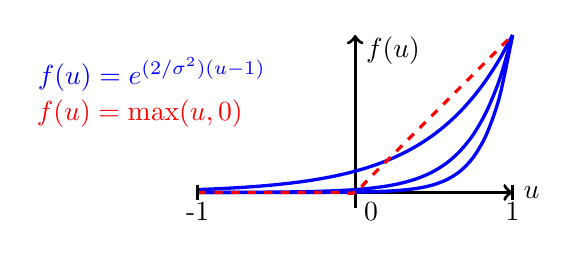
\begin{tikzpicture}[scale=2]
      \draw[->,very thick,black] (-1,0) -- (1,0) node[right] {$u$};
      \draw[->,very thick,black] (0,-0.1) -- (0,1) node[right,yshift=-2mm] {$f(u)$};
      \draw[scale=1,domain=-1:1,smooth,variable=\x,very thick,blue] plot ({\x},{exp(2*(\x-1))});
      \draw[scale=1,domain=-1:1,smooth,variable=\x,very thick,blue] plot ({\x},{exp(4*(\x-1))}) node[left,xshift=-3cm,yshift=-0.5cm] {$f(u)=e^{(2/\sigma^2)(u-1)}$};
      \draw[scale=1,domain=-1:1,smooth,variable=\x,very thick,blue] plot ({\x},{exp(6*(\x-1))});
      \draw[scale=1,domain=-1:1,smooth,variable=\x,very thick,dashed,red] plot ({\x},{max(\x,0)}) node[left,xshift=-3.29cm,yshift=-1cm] {$f(u)=\max(u,0)$};
      \draw (0,0) node[anchor=north,xshift=2mm] {0};
      \draw (1,0) node[anchor=north] {1};
      \draw (-1,0) node[anchor=north] {-1};
      \draw[very thick] (-1,0.05) -- (-1,-0.05);
      \draw[very thick] (1,0.05) -- (1,-0.05);
   \end{tikzpicture}
   \vspace*{-0.3cm}
   \caption{In dotted red, we plot the ``rectified linear unit'' function $u \mapsto \max(u,0)$. In blue, we plot non-linear functions of our network for typical values of~$\sigma$ that we use in our experiments.}\label{fig:relu}
\end{figure}

\vspace*{-0.3cm}
\subsection{Approximating the Multilayer Convolutional Kernel}

We have now all the tools in hand to build our convolutional kernel network.
We start by making assumptions on the input data, and then present the learning scheme and its approximation principles.

\vs
\paragraph{The zeroth layer.} We assume that the input data is a
finite-dimensional map $\xi_0: \Omega_0' \to \Real^{p_0}$, and that $\varphi_0:
\Omega_0 \to \HH_0$ ``extracts'' patches from~$\xi_0$. Formally, there
exists a patch shape~$\PP_0'$ such that $\Omega_0' = \Omega_0 + \PP_0'$, $\HH_0
= \Real^{p_0|\PP_0'|}$, and for all $\z_0$ in~$\Omega_0$, $\varphi_0(\z_0)$ is
a patch of $\xi_0$ centered at~$\z_0$. 
Then, property {\bfseries (B)} described at the beginning of
Section~\ref{sec:approx} is satisfied for $k\!=\!0$ by choosing
$\psi_0\!=\!\varphi_0$. The examples of input feature maps given earlier
satisfy this finite-dimensional assumption: for the gradient map, $\xi_0$ is
the gradient of the image along each direction, with $p_0=2$, $\PP_0'=\{ 0\}$
is
a $1 \!\times \!1$ patch, $\Omega_0\!=\!\Omega_0'$, and $\varphi_0\!=\!\xi_0$;
for the patch map, $\xi_0$ is the input image, say with $p_0\!=\!3$ for RGB data.


\vs
\paragraph{The convolutional kernel network.}
The zeroth layer being characterized, we present in Algorithms~\ref{alg:ckn}
and~\ref{alg:ckn2} the subsequent layers and how to learn their parameters 
in a feedforward manner. It is interesting to note that the input parameters of
the algorithm are exactly the same as a CNN---that is, number of layers and filters,
sizes of the patches and feature maps (obtained here via the subsampling factor).
Ultimately, CNNs and CKNs only differ in the cost function that is
optimized for learning the filters and in the choice of non-linearities.  As we
show next, there exists a link between the parameters of a CKN and those of
a convolutional multilayer kernel.

\begin{algorithm}
   \caption{Convolutional kernel network - learning the parameters of the $k$-th layer.}\label{alg:ckn}
   \begin{algorithmic}[1]
      \INPUT $\xi^1_{\kmone}, \xi^2_{\kmone},\ldots: \Omega'_{\kmone} \to \Real^{p_{\kmone}}$ (sequence of $(\kmone)$-th maps obtained from training images); $\PP_{\kmone}'$ (patch shape); $p_k$ (number of filters); $n$ (number of training pairs);
      \STATE extract at random $n$ pairs $(\x_i,\y_i)$ of patches with shape $\PP_{\kmone}'$ from the maps~$\xi_{\kmone}^1,\xi_{\kmone}^2,\ldots$;
      \STATE if not provided by the user, set $\sigma_k$ to the~$0.1$ quantile of the data~($\|\x_i-\y_i\|_2)_{i=1}^n$;
      \STATE {\bfseries unsupervised learning:} optimize~(\ref{eq:opt}) to obtain the filters~$\W_k$ in~$\Real^{|\PP_{\kmone}'|p_{\kmone} \times p_k}$ and $\etab_k$ in~$\Real^{p_k}$;
      \OUTPUT $\W_k$, $\etab_k$, and $\sigma_k$ (smoothing parameter);
   \end{algorithmic}
\end{algorithm}
\begin{algorithm}
   \caption{Convolutional kernel network - computing the $k$-th map form the~$(\kmone)$-th one.}\label{alg:ckn2}
   \begin{algorithmic}[1]
      \INPUT $\xi_{\kmone}: \Omega'_{\kmone} \!\to\! \Real^{p_{\kmone}}$ (input map); $\PP_{\kmone}'$ (patch shape); $\gamma_k \!\geq \!1$ (subsampling factor); $p_k$ (number of filters); $\sigma_k$ (smoothing parameter); $\W_k=[\w_{kl}]_{l=1}^{p_k}$ and~$\etab_k=[\eta_{kl}]_{l=1}^{p_k}$ (layer parameters);
      \STATE {\bfseries convolution and non-linearity:} define the activation map $\zeta_k: \Omega_{\kmone} \to \Real^{p_k}$ as
      \begin{equation}
         \vsb
         \zeta_k: \z \mapsto \|\psi_{\kmone}(\z)\|_2 \left[\sqrt{\eta_{kl}} e^{-\frac{1}{\sigma_k^2}\left\|\tildepsi_{\kmone}(\z)-\w_{kl}\right\|_2^2}\right]_{l=1}^{p_k}, \label{eq:zeta}
      \end{equation}
      where~$\psi_{\kmone}(\z)$ is a vector representing a patch from~$\xi_{\kmone}$ centered at~$\z$ with shape $\PP_{\kmone}'$, and the vector $\tildepsi_{\kmone}(\z)$ is an $\ell_2$-normalized version of~$\psi_{\kmone}(\z)$. This operation can be interpreted as a spatial convolution of the map~$\xi_{\kmone}$ with the filters~$\w_{kl}$ followed by pointwise non-linearities;
      \STATE set~$\beta_k$ to be~$\gamma_k$ times the spacing between two pixels in~$\Omega_{\kmone}$;
      \STATE {\bfseries feature pooling:}
      $\Omega'_k$ is obtained by subsampling~$\Omega_{\kmone}$ by a factor~$\gamma_k$ and we define a    
      new map $\xi_{k}: \Omega'_k \to \Real^{p_k}$ obtained from~$\zeta_k$ by linear pooling with Gaussian weights:
      \begin{equation}
         \vsb
         \xi_k: \z \mapsto \sqrt{{2}/\pi}\sum_{\u \in \Omega_{\kmone}}  e^{-\frac{1}{\beta_k^2}\left\|\u - \z\right\|_2^2} \zeta_k(\u). \label{eq:xi}
      \end{equation}
      \OUTPUT $\xi_{k} : \Omega'_k \to \Real^{p_k}$ (new map);
   \end{algorithmic}
\end{algorithm}

\paragraph{Approximation principles.}
\vspace*{-0.75cm}
We proceed recursively to show that the kernel approximation
property~{\bfseries (A)}
is satisfied; we assume that~{\bfseries (B)}
holds at layer~$\kmone$, and then, we show that {\bfseries (A)} and
{\bfseries (B)} also hold at layer~$k$.  This is sufficient for our 
purpose since we have previously assumed~{\bfseries (B)} for the zeroth layer.  
Given two images feature maps~$\varphi_{\kmone}$ and~$\varphi_{\kmone}'$, we 
start by approximating $K(\varphi_{\kmone},\varphi_{\kmone}')$ by replacing
$\varphi_{\kmone}(\z)$ and $\varphi_{\kmone}'(\z')$ by their finite-dimensional
approximations provided by~{\bfseries (B)}: 
\begin{equation}
   K(\varphi_{\kmone},\varphi_{\kmone}') \approx 
   \sum_{\z,\z' \in \Omega_{\kmone}} \normE{\psi_{\kmone}(\z)}  \normE{\psi_{\kmone}'(\z')} e^{-\frac{1}{2\beta_{k}^2}\normE{\z-\z'}^2} e^{-\frac{1}{2\sigma_k^2} \normE{\tildepsi_{\kmone}(\z)-\tildepsi_{\kmone}'(\z')}^2}.
\end{equation}
Then, we use the finite-dimensional approximation of the Gaussian kernel
involving~$\sigma_k$ and
\begin{equation}
         \vsb
   K(\varphi_{\kmone},\varphi_{\kmone}') \approx 
   \sum_{\z, \z' \in \Omega_{\kmone}} \zeta_k(\z)^\top \zeta_k'(\z') e^{-\frac{1}{2\beta_k^2}\normE{\z-\z'}^2},
\end{equation}
where~$\zeta_k$ is defined in~(\ref{eq:zeta}) and $\zeta_k'$ is defined
similarly by replacing~$\tildepsi$ by~$\tildepsi'$.  Finally, we approximate
the remaining Gaussian kernel by uniform sampling on $\Omega_{k}'$,
following Section~\ref{subsec:approx_gaussian}.
After exchanging sums and grouping appropriate terms together, we obtain the new approximation 
\begin{equation}
   K(\varphi_{\kmone},\varphi_{\kmone}') \approx \frac{2}{\pi} \sum_{\u \in \Omega_{k}'} \bigg( \sum_{\z \in \Omega_{\kmone}} e^{-\frac{1}{\beta_k^2}\normE{\z-\u}^2}\zeta_k(\z) \bigg)^\top \bigg( \sum_{\z' \in \Omega_{\kmone}}  e^{-\frac{1}{\beta_k^2}\normE{\z'-\u}^2} \zeta_k'(\z')  \bigg), \label{eq:approx}
\end{equation}
where the constant~$2/\pi$ comes from the multiplication of the constant
$2/(\pi\beta_k^2)$ from~(\ref{eq:rbf}) and the weight $\beta_k^2$ of uniform sampling
orresponding to the square of the distance between two pixels
of~$\Omega_k'$.\footnote{The choice of~$\beta_k$ in Algorithm~\ref{alg:ckn2} is
driven by signal processing principles. The feature pooling step can indeed be
interpreted as a downsampling operation that reduces the resolution of the map
from~$\Omega_{\kmone}$ to~$\Omega_k$ by using a Gaussian anti-aliasing filter,
whose role is to reduce frequencies
above the Nyquist limit.} As a result, the right-hand side is exactly $\langle
\xi_{k}, \xi_k' \rangle$, where~$\xi_k$ is defined in~(\ref{eq:xi}), giving us
property~{\bfseries (A)}. It remains to show that property~{\bfseries (B)} also
holds, specifically that the quantity~(\ref{eq:kernelpatch}) can be
approximated by the Euclidean inner-product~$\langle\psi_{k}(\z_k),
\psi'_k(\z_k')\rangle$ with the patches~$\psi_k(\z_k)$ and~$\psi'_k(\z_k')$ of shape~$\PP_k'$; we assume for that purpose that~$\PP_k'$ is a
subsampled version of the patch shape~$\PP_k$ by a factor~$\gamma_k$.

We remark that the kernel~(\ref{eq:kernelpatch}) is the same
as~(\ref{eq:kernel}) applied to layer~$\kmone$ by replacing~$\Omega_{\kmone}$
by~$\{\z_k\}+\PP_k$. By doing the same substitution in~(\ref{eq:approx}), we
immediately obtain an approximation of~(\ref{eq:kernelpatch}). Then, all
Gaussian terms are negligible for all~$\u$ and~$\z$ that are far from each
other---say when $\|\u-\z\|_2 \geq 2\beta_k$. Thus, we may replace the
sums~$\sum_{\u \in \Omega_k'}\sum_{\z,\z' \in \{\z_k\}+\PP_k}$ by~$\sum_{\u \in \{\z_k\}+\PP_k'}\sum_{\z,\z' \in \Omega_{\kmone}}$,
which has the same set of ``non-negligible'' terms. This yields exactly the
approximation $\langle\psi_{k}(\z_k), \psi'_k(\z_k')\rangle$.

\vs
\paragraph{Optimization.} 
Regarding problem~(\ref{eq:opt}), stochastic gradient descent
(SGD) may be used since a potentially infinite amount of training
data is available. However, we have preferred to use
L-BFGS-B~\cite{byrd1995} on $300\,000$ pairs of randomly selected training data
points, and initialize~$\W$ with the K-means algorithm. L-BFGS-B
is a parameter-free state-of-the-art batch method, which is not as
fast as SGD but much easier to use. We always run the L-BFGS-B algorithm for~$4\,000$ iterations, which seems to ensure
convergence to a stationary point. Our goal is to demonstrate the preliminary
performance of a new type of convolutional network, and we leave as future work
any speed improvement. 
\vsb


\section{Experiments}\label{sec:exp}
\section{Evaluation}
In this section, we present a comparative performance evaluation of our proposed method.
Specifically, we conduct experiments on the widely-used fine-grained benchmark Caltech-UCSD birds dataset \cite{DatasetCUB200} (CUB200-2011).
The classification task is to discriminate among 200 species of birds, and is challenging for computer vision systems due to the high degree of similarity between categories.
It contains 11,788 images of 200 bird species. Each image is annotated with its bounding box and the image coordinates of fifteen keypoints: the beak, back, breast, belly, forehead, crown, left eye, left leg, left wing, right eye, right leg, right wing, tail, nape and throat. We train and test on the splits included with the dataset, which contain around 30 training samples for each species.
Following the protocol of \cite{dpd}, we use two semantic parts for the bird dataset: head and body.
%Figure~\ref{fig:ningfig} (left) illustrates the set of keypoints which comprise the head part, and Figure~\ref{fig:ningfig} (right) illustrates the body part.

We use the open-source package Caffe~\cite{Jia13caffe} to extract deep features and fine-tune our CNNs. For object and part detections, we use the Caffe reference model, which is almost identical to the model used by Krizhevsky et al. in \cite{krizhevsky}. We refer deep features from each layer as \texttt{conv}$n$, \texttt{pool}$n$, or \texttt{fc}$n$ for the $n$th layer of the CNN, which is the output of a convolutional,
pooling, or fully connected layer respectively.
We use \texttt{fc6} to train R-CNN object and part detectors as well as image representation for classification.
%We use \texttt{fc6} to train R-CNN object and part detectors as well as image representation for classification, except in the experiments using fine-tuned networks where \texttt{fc7} features are used, as these features are directly optimized for input into a linear classifier on the target bird classification task.
For $\delta^{NP}$, nearest neighbors are computed using \texttt{pool5}  and cosine distance metric.


\subsection{Fine-grained categorization}
We first present results on the standard fine-grained categorization task associated with the Caltech-UCSD birds dataset.
The first set of results in Table~\ref{tab:finegrainedres} are achieved in the setting where the ground truth bounding box for the entire bird is known at test time, as most state-of-art methods assume, making the categorization task somewhat easier. 
In this setting, our part-based method with the local non-parametric geometric constraint $\delta^{NP}$ works the best without fine-tuning, achieving 68.1\% classification accuracy without fine-tuning.
Fine-tuning improves this result by a large margin, to over 76\%.
We compare our results against three state-of-the-art baseline approaches with results assuming the ground truth bounding box at test time. We use deep convolutional features as the authors of \cite{decaf}, but they use a HOG-based DPM as their part localization method. The increase in performance is likely due to better part localization (see Table \ref{tab:partlocalres}). Oracle method uses the ground truth bounding box and part annotations for both training and test time. 

The second set of results is in the less artificial setting where the bird bounding box is \emph{unknown} at test time. Most of the literature on this dataset doesn't  report performance in this more difficult, but more realistic setting. As Table \ref{tab:finegrainedres} shows, in this setting our part-based method works much better than the baseline DPD model. We achieve 66.0\% classification accuracy without finetuning , almost as good as the accuracy we can achieve when the ground truth bounding box is given. This means there is no need to annotate any box during test time to classify the bird species. With finetuned CNN models, our method achieves 73.89\% classification accuracy. 
We are unaware of any other published results in this more difficult setting, but we note that our method outperforms previous state-of-the-art even without knowledge of the ground truth bounding box.

Another interesting experiment we did is to remove the part descriptors by only looking at the image descriptors inside the predicted bounding box. By having geometric constraints over part locations relative to object location, our method is able to help localize the object. As Table \ref{tab:finegrained_noparts} shows, our method outperforms a single object detector using R-CNN, which means the geometric constraints helps our method better localize the object window. The detection of strong DPM is not as accurate as our method, which explains the performance drop.
The ``oracle'' method uses the ground truth bounding box and achieves 57.94\% accuracy, which is still much lower than the method in Table \ref{tab:finegrainedres} of using both image descriptors inside object and parts.


\begin{table}[t]
\centering
\caption{Fine-grained categorization results on CUB200-2011 bird dataset. -ft means extracting deep features from finetuned CNN models using each semantic part. Oracle method uses the ground truth bounding box and part annotations for both training and test time. } 
\begin{tabular}{|l|r|}
\hline
\multicolumn{2}{|c|}{Bounding Box Given} \\
\hline
DPD~\cite{dpd} & 50.98\% \\
DPD+DeCAF feature ~\cite{decaf} & 64.96\% \\
POOF~\cite{poof} & 56.78\% \\
Symbiotic Segmentation~\cite{iccv13_symbiotic} & 59.40\% \\
Alignment~\cite{iccv13_alignment} & 62.70\%\\
\hline
Oracle & 72.83\% \\
Oracle-ft & 82.02\%\\
\hline
Ours ($\Delta_{\mathrm{box}}$) & 67.55\% \\
Ours ($\Delta_{\mathrm{geometric}}$ with $\delta^{MG}$) & 67.98\% \\
Ours ($\Delta_{\mathrm{geometric}}$ with $\delta^{NP}$) & 68.07\% \\
Ours-ft ($\Delta_{\mathrm{box}}$) & 75.34\% \\
Ours-ft ($\Delta_{\mathrm{geometric}}$ with $\delta^{MG}$) &  \textbf{76.37\%}\\
Ours-ft ($\Delta_{\mathrm{geometric}}$ with $\delta^{NP}$) & 76.34\%\\
\hline
\hline
\multicolumn{2}{|c|}{Bounding Box Unknown} \\
\hline
DPD+DeCAF~\cite{decaf} with no bounding box & 44.94\% \\
Ours ($\Delta_{\mathrm{null}}$) & 64.57\% \\
Ours ($\Delta_{\mathrm{box}}$)& 65.22\% \\
Ours ($\Delta_{\mathrm{geometric}}$ with $\delta^{MG}$) &65.98\% \\
Ours ($\Delta_{\mathrm{geometric}}$ with $\delta^{NP}$) & 65.96\% \\
Ours-ft ($\Delta_{\mathrm{box}}$)& 72.73\% \\
Ours-ft ($\Delta_{\mathrm{geometric}}$ with $\delta^{MG}$) & 72.95\% \\
Ours-ft ($\Delta_{\mathrm{geometric}}$ with $\delta^{NP}$) & \textbf{73.89\%} \\
\hline
\end{tabular}
\label{tab:finegrainedres}
\end{table}

\begin{table}[t]
\centering
\caption{Fine-grained categorization results on CUB200-2011 bird dataset with \emph{no parts}. We trained a linear SVM using deep features on all the methods. Therefore only the bounding box prediction is the factor of difference. -ft is the result of extracting deep features from fine-tuned CNN model on bounding box patches. } \label{tab:finegrained_noparts}
\begin{tabular}{|l|r|}
\hline
Oracle (ground truth bounding box) & 57.94\%\\
Oracle-ft & 68.29\% \\
\hline 
Strong DPM \cite{Hossein_ECCV12} & 38.02\% \\
R-CNN~\cite{rcnn} & 51.05\% \\
\hline \hline
Ours ($\Delta_{\mathrm{box}}$)  & 50.17\% \\
Ours ($\Delta_{\mathrm{geometric}}$ with $\delta^{MG}$) & 51.83\% \\
Ours ($\Delta_{\mathrm{geometric}}$ with $\delta^{NP}$) & 52.38\%\\
Ours-ft ($\Delta_{\mathrm{box}}$)  &  62.13\%\\
Ours-ft ($\Delta_{\mathrm{geometric}}$ with $\delta^{MG}$) & 62.06\% \\
Ours-ft ($\Delta_{\mathrm{geometric}}$ with $\delta^{NP}$) & \textbf{62.75\%} \\
\hline
\end{tabular}
\end{table}

\subsection{Part localization}
We now present results evaluating in isolation the ability of our system to accurately localize parts.
Our results in Table~\ref{tab:partlocalres} are given in terms of the Percentage of Correctly Localized Parts (PCP) metric. 
For the first set of results, the whole object bounding box is given and the task is simply to correctly localize the parts inside of this bounding box, with parts having $\ge 0.5$ overlap with ground truth counted as correct.

For the second set of results, the PCP metric is computed on top-ranked parts predictions using the objective function described in Sec. 3.2.
Note that in this more realistic setting we do not assume knowledge of the ground truth bounding box at test time -- despite this limitation, our system produces accurate part localizations.
% It is worthy to note that we don't have any assumption that the object bounding box prediction having at least 0.5 overlap with the ground truth bounding box, as some other methods suggested.
% The main point is to show without any knowledge of bounding box at test time, our system is able to produce accurate part localizations. 

\begin{table}[t]
\centering
\caption{Recall of region proposals produced by selective search methods on CUB200-2011 bird dataset. We use ground truth part annotations to compute the recall, as defined by the proportion of ground truth boxes for which there exists a region proposal with overlap at least 0.5, 0.6 and 0.7 respectively.}\label{tab:selective_search_recall}
\begin{tabular}{|c|c|c|c|}
\hline
%\multicolumn{4}{|c|}{Bounding Box Given} \\
%\hline
%Overlap & 0.50 & 0.60 & 0.70\\
%\hline
%Head & 94.71\% &  & \\
%Body & 97.39\%  & & \\
%\hline
%\multicolumn{4}{|c|}{Bounding Box Unknown} \\
%\hline
Overlap & 0.50 & 0.60 & 0.70\\
\hline
Bounding box & 96.70\% & 97.68\% & 89.50\% \\
Head &  93.34\% & 73.87\%& 37.57\%\\
Body & 96.70\% & 85.97\%&54.68\%\\
\hline
\end{tabular}
\end{table}

\begin{table}[t]
\centering
\caption{Part localization accuracy in terms of PCP (Percentage of Correctly Localized Parts) on the CUB200-2011 bird dataset. There are two different settings: with given bounding box and without bounding box. } 
\label{tab:partlocalres}
\begin{tabular}{|l|r|r|}
\hline
\multicolumn{3}{|c|}{Bounding Box Given} \\
\hline
& \multicolumn{1}{|c|}{Head}
& \multicolumn{1}{|c|}{Body}
\\
\hline
Strong DPM~\cite{Hossein_ECCV12} & 43.49\% & 75.15\% \\
Ours ($\Delta_{\mathrm{box}}$)   & 61.40\% & 65.42\% \\
Ours ($\Delta_{\mathrm{geometric}}$ with $\delta^{MG}$)& 66.03\% & 76.62\% \\
Ours ($\Delta_{\mathrm{geometric}}$ with $\delta^{NP}$) & \textbf{68.19\%} & \textbf{79.82\%} \\
\hline
\multicolumn{3}{|c|}{Bounding Box Unknown} \\
\hline
& \multicolumn{1}{|c|}{Head}
& \multicolumn{1}{|c|}{Body}
\\
\hline
Strong DPM~\cite{Hossein_ECCV12} & 37.44\% & 47.08\% \\
Ours ($\Delta_{\mathrm{null}}$  ) &60.50\% &  64.43\% \\
Ours ($\Delta_{\mathrm{box}}$)  & 60.56\% & 65.31\% \\
Ours ($\Delta_{\mathrm{geometric}}$ with $\delta^{MG}$)& \textbf{61.94\%} & 70.16\% \\ 
Ours ($\Delta_{\mathrm{geometric}}$ with $\delta^{NP}$) & 61.42\% & \textbf{70.68\%} \\
\hline
\end{tabular}
\end{table}

\begin{figure*}[t]
\begin{center}
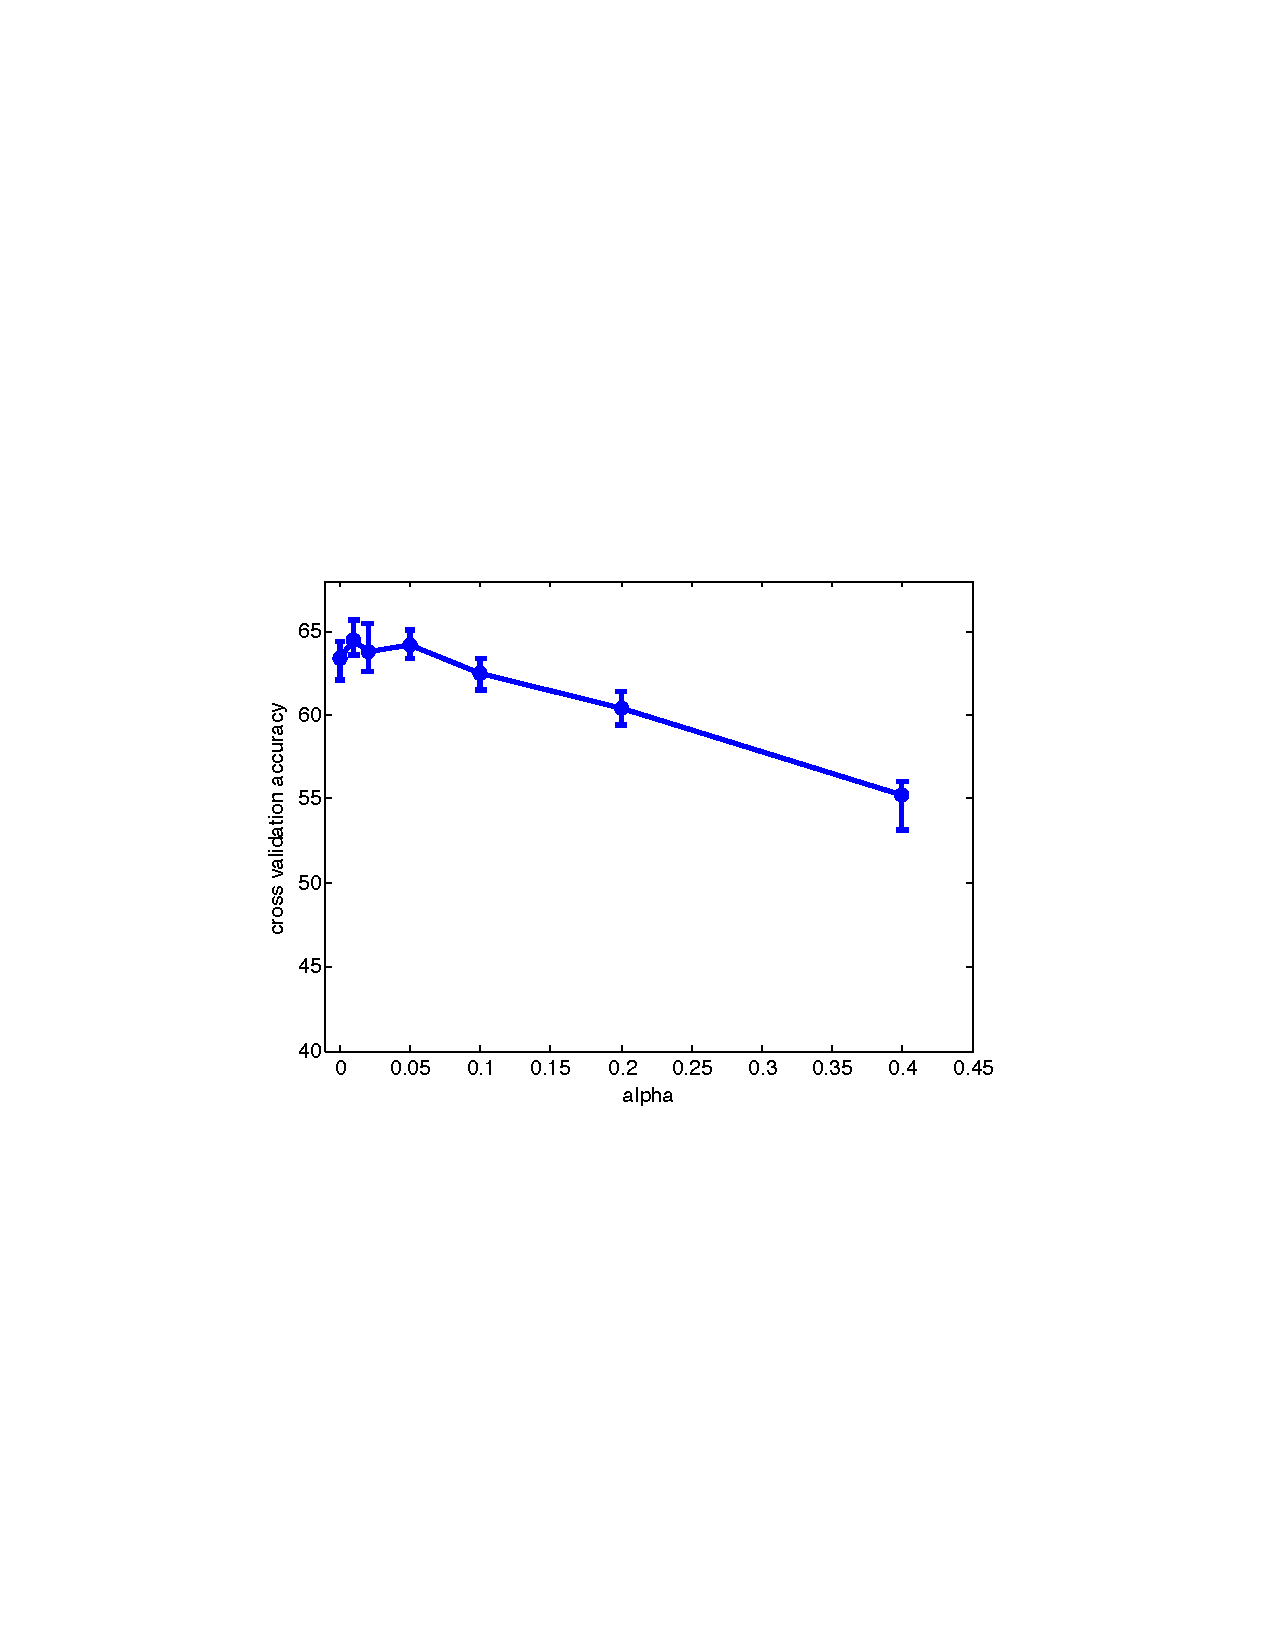
\includegraphics[width=0.45\linewidth]{alpha_plot.pdf}
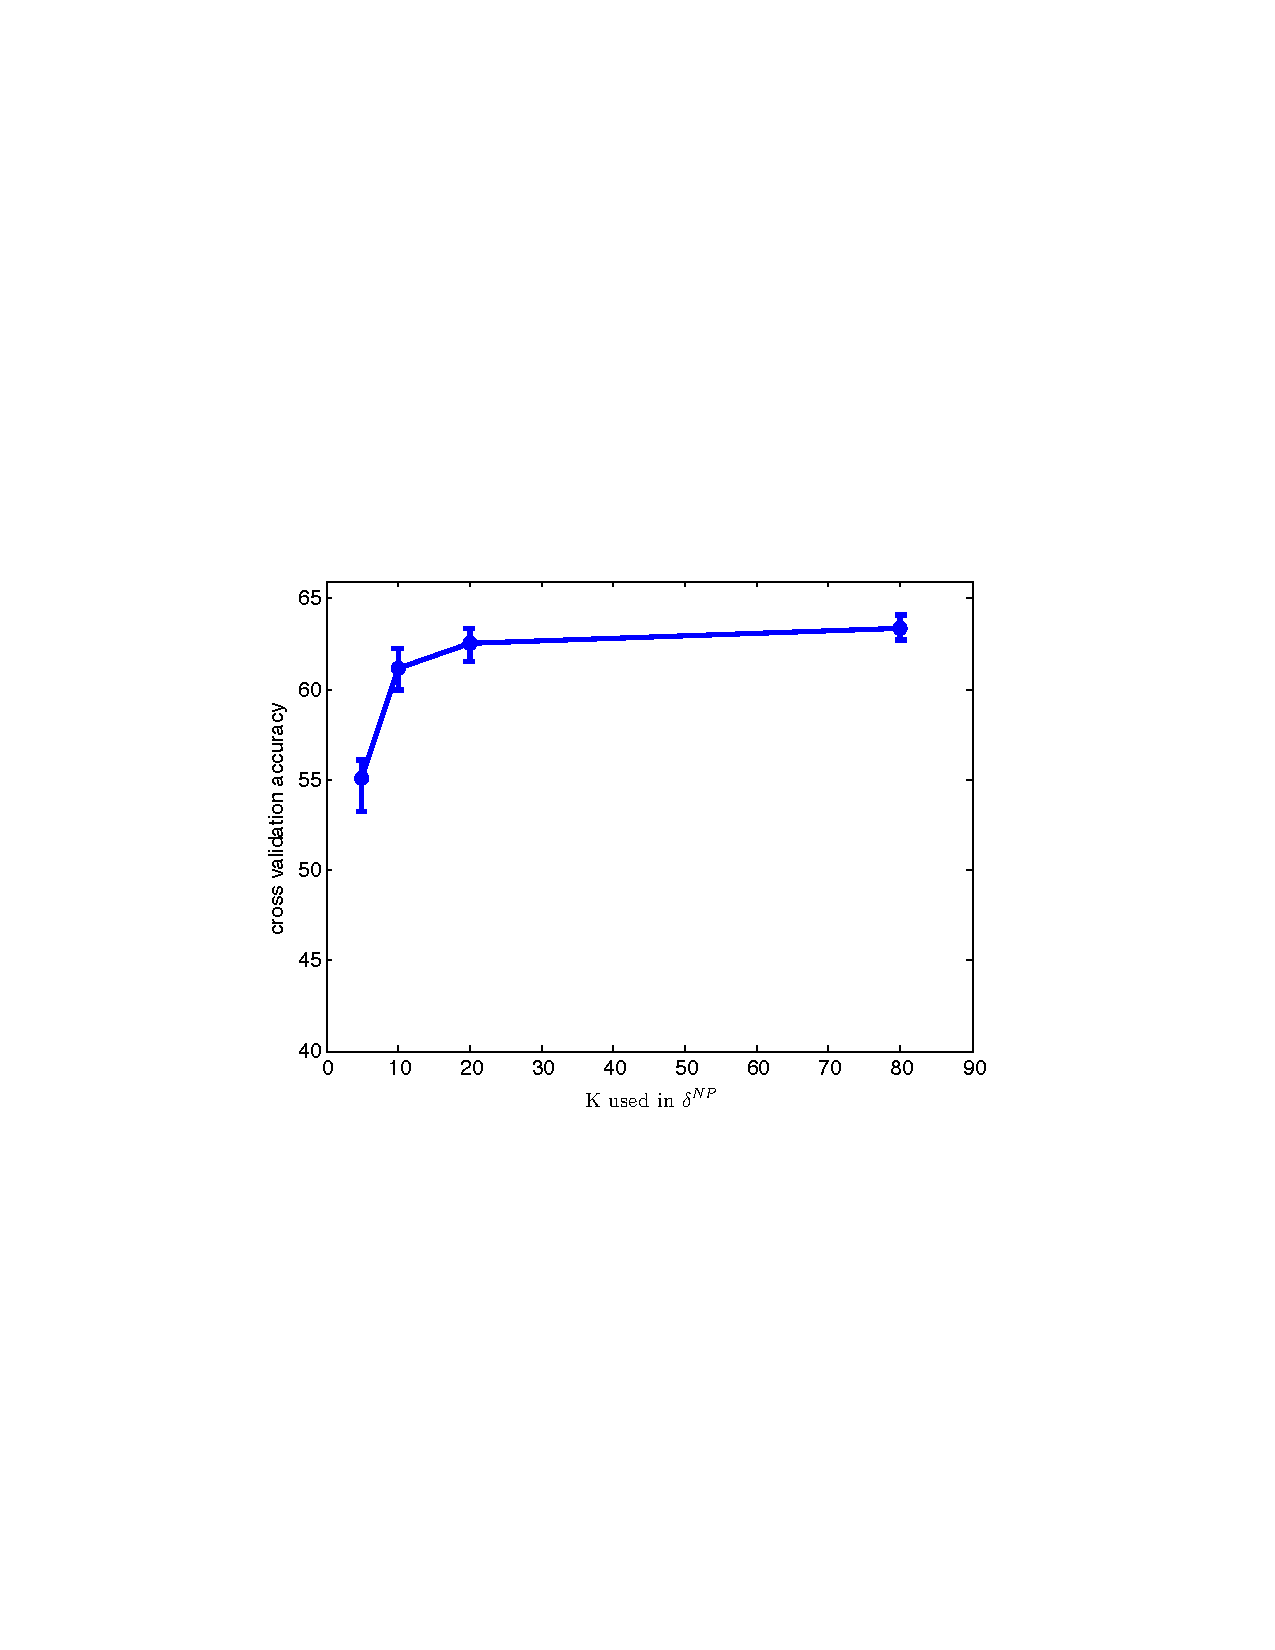
\includegraphics[width=0.45\linewidth]{K_plot.pdf}
\end{center}
\caption{Cross-validation results on fine-grained accuracy for different values of $\alpha$ (left) and $K$ (right). We split the training data into 5 folds and use cross-validate each hyperparameter setting.}
\label{fig:crossvalidationalphak}
\end{figure*}




As shown in Table \ref{tab:partlocalres}, for both settings of given bounding box and unknown bounding box, our methods outperform the strong DPM~\cite{Hossein_ECCV12} method.
Adding a geometric constraint $\delta^{NP}$ improves our results (79.82\% for body localization compared to 65.42\%). In the fully automatic setting, the top ranked detection and part localization performance on head is 65\% better than the baseline method. $\Delta_{\mathrm{null}}=1$ is the appearance-only case with no geometric constraints applied. Although the fine-grained classification results don't show a big gap between $\Delta_{\mathrm{geometric}}$ and $\Delta_{\mathrm{box}}$, we can see the performance gap for part localization.
The reason for the small performance gap might be that deep convolutional features are invariant to small translations and rotations,
limiting the impact of small localization errors on our end-to-end accuracy.


We also evaluate the recall performance of selective search region proposals \cite{selsearch} for bounding box and semantic parts. 
The results of recall given different overlapping thresholds are shown in Table \ref{tab:selective_search_recall}. 
Recall for the bird head and body parts is high when the overlap requirement is $0.5$, which provides the foundation for localizing these parts given the region proposals. However, we also observe that the recall for head is below $40\%$ when the overlap threshold is $0.7$, indicating the bottom-up region proposals could be a bottleneck for precise part localization.

Other visualizations are shown in Figure~\ref{fig:comparasion}. We show three detection and part localization for each image, the first column is the output from strong DPM, the second column is our methods with individual part predictions and the last column is our method with local prior. We used the model pretrained from \cite{Hossein_ECCV12} to get the results. We also show some failure cases of our method in Figure~\ref{fig:failure}.


\subsection{Component Analysis}
To examine the effect of different values of $\alpha$ and $K$ used in $\Delta_{\mathrm{geometric}}$, we conduct cross-validation experiments.
Results are shown in Figure~\ref{fig:crossvalidationalphak}. We fix $K=20$ in Figure~\ref{fig:crossvalidationalphak}, left and fix $\alpha = 0.1$ in Figure \ref{fig:crossvalidationalphak}, right. All the experiments on conducted on training data in a cross-validation fashion and we split the training data into 5 folds.
%\todo{can we add error bars? ... if you still have the results}.
As the results show, the end-to-end fine-grained classification results are sensitive to the choice of $\alpha$ and $\alpha=0$ is the case of $\Delta_{\mathrm{box}}$ predictions without any geometric constraints. The reason why we have to pick a small $\alpha$ is the pdf of the Gaussian is large compared to the logistic score function output from our part detectors. On the other hand, the choice of $K$ cannot be too small and it is not very sensitive when $K$ is larger than 10. 


%Experiment results vary K, vary $\alpha$
%Answer the following questions,
%1) Are parts necessary, show results with only root filter
%2) Are neighbors necssarcy, show only fit into one Gaussian
%3) Show hor prior helps, show results without prior
%
%figure to visualize the prior over neighbors v.s. prior over the whole training data


\begin{figure*}
\begin{center}
\begin{tabular}{ccc}
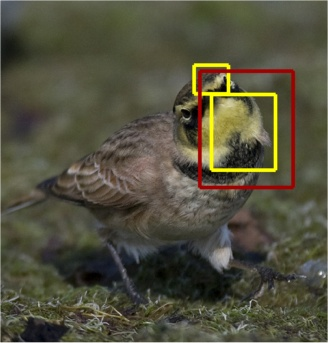
\includegraphics[width=0.3\linewidth]{6_strong_dpm.jpg} &
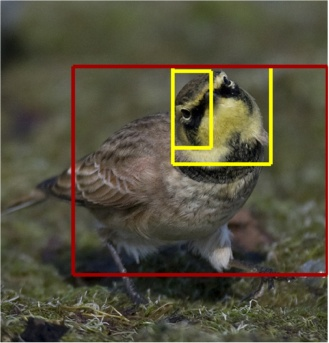
\includegraphics[width=0.3\linewidth]{6_individual.jpg} &
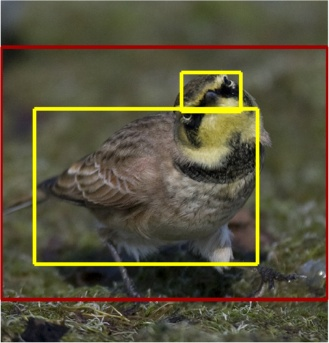
\includegraphics[width=0.3\linewidth]{6_neighbor.jpg} \\
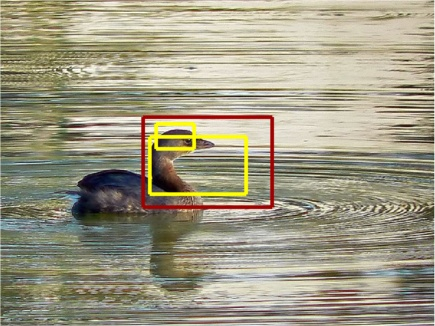
\includegraphics[trim=0mm 10mm 0mm 10mm, clip, width=0.3\linewidth]{11_strong_dpm.jpg} &
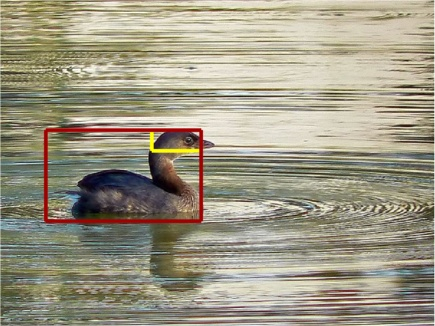
\includegraphics[trim=0mm 10mm 0mm 10mm, clip, width=0.3\linewidth]{11_individual.jpg} &
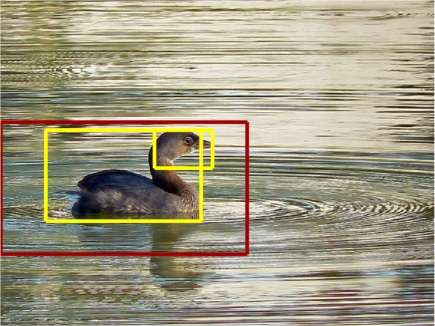
\includegraphics[trim=0mm 10mm 0mm 10mm, clip, width=0.3\linewidth]{11_neighbor.jpg} \\
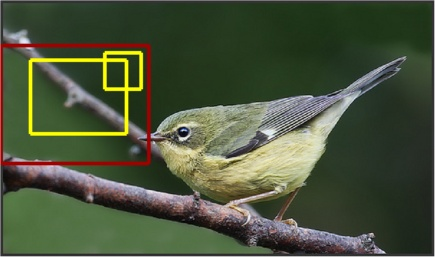
\includegraphics[width=0.3\linewidth]{13_strong_dpm.jpg} &
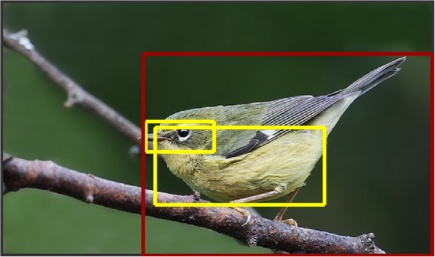
\includegraphics[width=0.3\linewidth]{13_individual.jpg} &
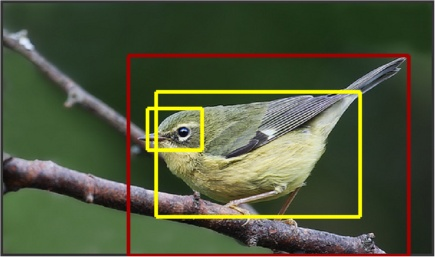
\includegraphics[width=0.3\linewidth]{13_neighbor.jpg} \\
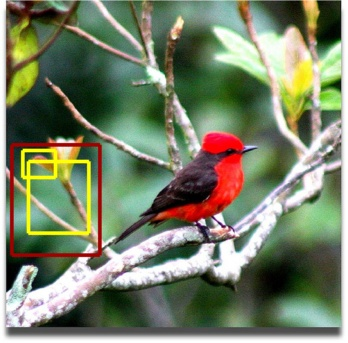
\includegraphics[trim=0mm 20mm 0mm 20mm, clip, width=0.3\linewidth]{15_strong_dpm.jpg} &
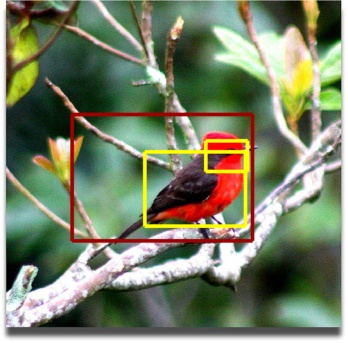
\includegraphics[trim=0mm 20mm 0mm 20mm, clip, width=0.3\linewidth]{15_individual.jpg} &
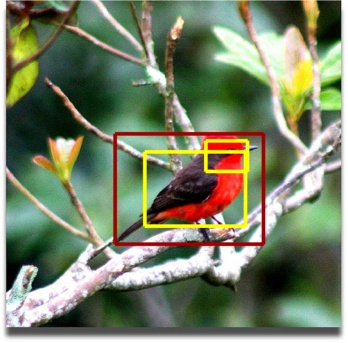
\includegraphics[trim=0mm 20mm 0mm 20mm, clip, width=0.3\linewidth]{15_neighbor.jpg} \\
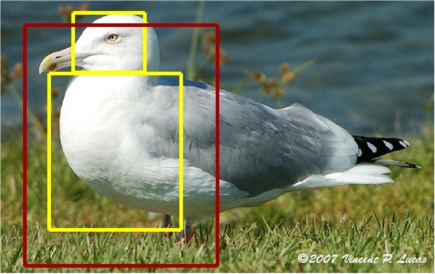
\includegraphics[width=0.3\linewidth]{16_strong_dpm.jpg} &
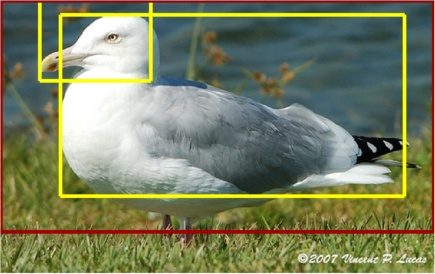
\includegraphics[width=0.3\linewidth]{16_individual.jpg} &
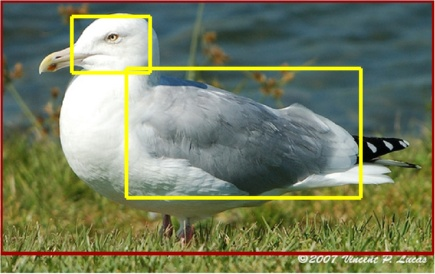
\includegraphics[width=0.3\linewidth]{16_neighbor.jpg} \\
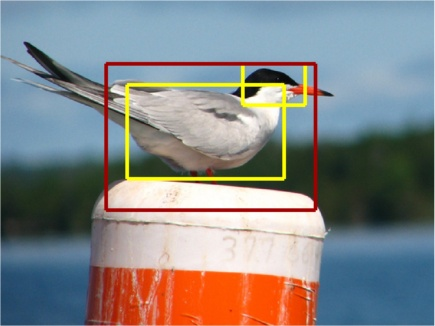
\includegraphics[width=0.3\linewidth]{17_strong_dpm.jpg} &
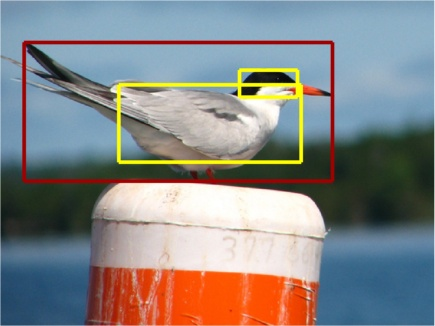
\includegraphics[width=0.3\linewidth]{17_individual.jpg} &
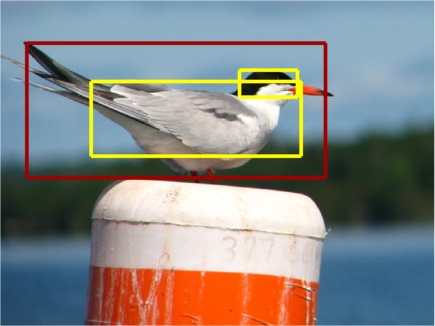
\includegraphics[width=0.3\linewidth]{17_neighbor.jpg} \\
% 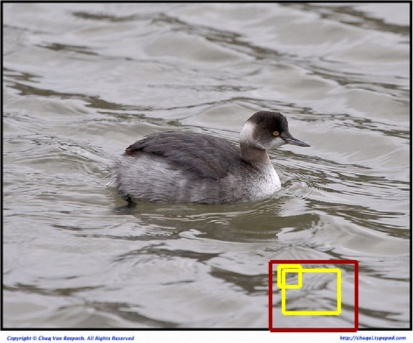
\includegraphics[width=0.3\linewidth]{19_strong_dpm.jpg} &
% 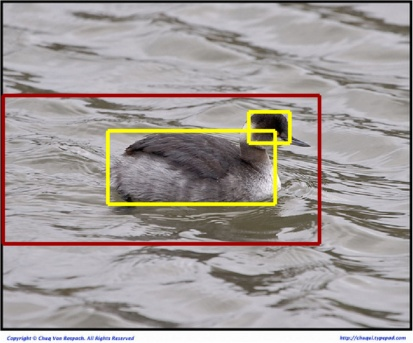
\includegraphics[width=0.3\linewidth]{19_individual.jpg} &
% 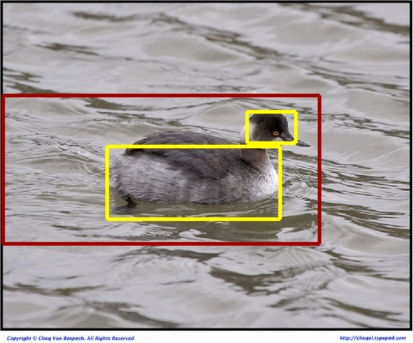
\includegraphics[width=0.3\linewidth]{19_neighbor.jpg} \\
% 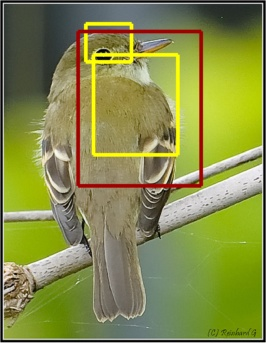
\includegraphics[width=0.3\linewidth]{30_strong_dpm.jpg} &
% 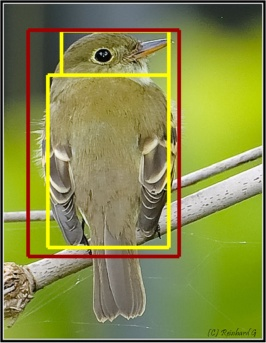
\includegraphics[width=0.3\linewidth]{30_individual.jpg} &
% 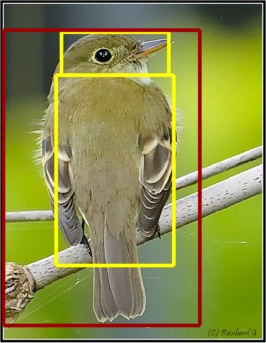
\includegraphics[width=0.3\linewidth]{30_neighbor.jpg} \\
Strong DPM & Ours ($\Delta_{box}$) & Ours ($\delta^{NP}$)
\\
\end{tabular}
\end{center}
\caption{{Examples of bird detection and part localization from strong DPM~\cite{Hossein_ECCV12} (left); our method using $\Delta_{\mathrm{box}}$ part predictions (middle); and our method using $\delta^{NP}$(right). All detection and localization results without any assumption of bounding box. }}
\label{fig:comparasion}
\end{figure*}

\begin{figure*}
\begin{center}
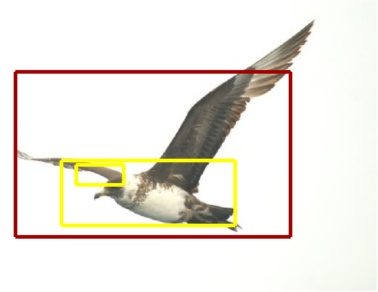
\includegraphics[height=0.2\linewidth]{8_neighbor.jpg} 
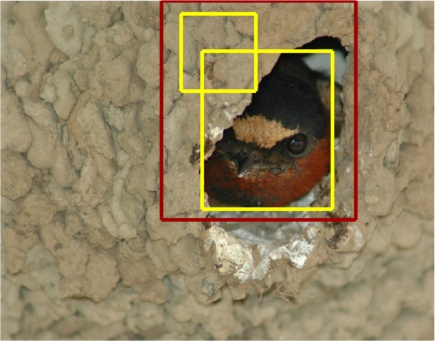
\includegraphics[height=0.2\linewidth]{32_neighbor.jpg} 
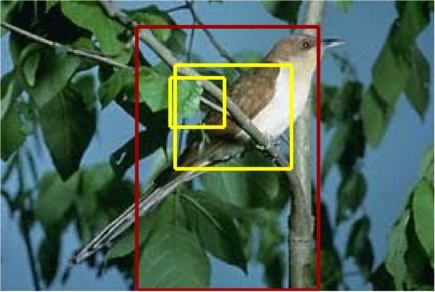
\includegraphics[height=0.2\linewidth]{41_neighbor.jpg} 
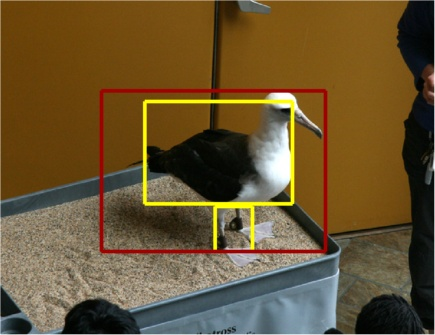
\includegraphics[height=0.2\linewidth]{57_neighbor.jpg} 
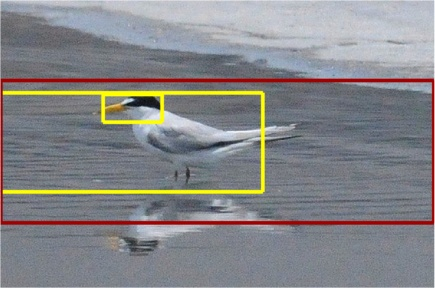
\includegraphics[height=0.2\linewidth]{58_neighbor.jpg}
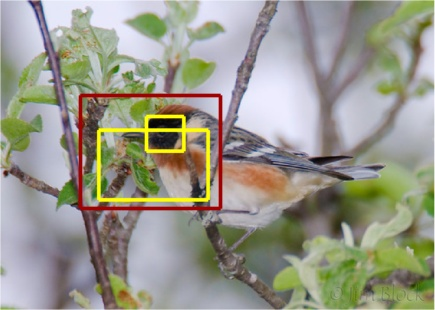
\includegraphics[height=0.2\linewidth]{64_neighbor.jpg} 
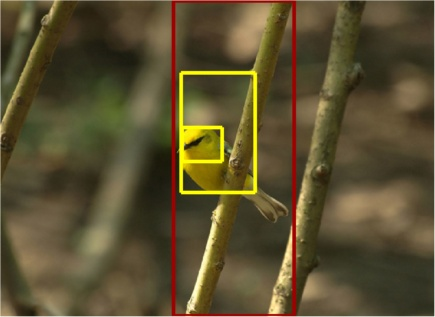
\includegraphics[height=0.2\linewidth]{99_neighbor.jpg} 
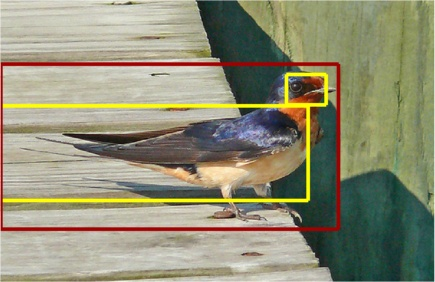
\includegraphics[height=0.2\linewidth]{47_neighbor.jpg} 
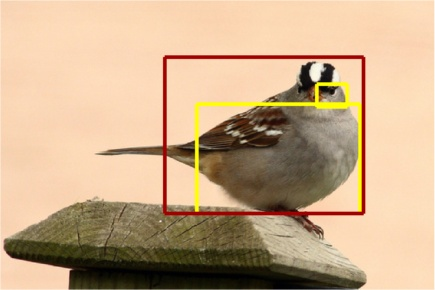
\includegraphics[height=0.2\linewidth]{91_neighbor.jpg} 
\end{center}
\caption{{Failure cases of our part localization using $\delta^{NP}$.}}
\label{fig:failure}
\end{figure*}


\vs
\section{Conclusion}\label{sec:ccl}
\vsb
In this paper, we have proposed a new methodology for combining kernels
and convolutional neural networks. We show that  
mixing the ideas of these two concepts is fruitful,
since we achieve near state-of-the-art performance 
on several datasets such as MNIST, CIFAR-10, and STL10, with simple architectures
and no data augmentation.
Some challenges regarding our work are left open for the future. The first one
is the use of supervision to better approximate the kernel for the prediction
task. The second consists in leveraging the kernel interpretation of our
convolutional neural networks to better understand the theoretical properties
of the feature spaces that these networks produce.



\vsb
\subsubsection*{Acknowledgments}
\vsb
This work was partially supported by grants from ANR (project MACARON ANR-14-CE23-0003-01),
MSR-Inria joint centre, European Research Council (project ALLEGRO), CNRS-Mastodons program (project GARGANTUA), and the LabEx PERSYVAL-Lab (ANR-11-LABX-0025).

\newpage
\small{
   \bibliographystyle{plain}
   \bibliography{abbrev,main}
}
 \appendix
 %%%%%%%%%%%%%%%%%%%%%%%%%%%%%%%%%%%%%%%%%%%%%%%%%%%%%%%%%%%%%%
%%%%%%%%%%%%%%%%%%%% APPENDIX %%%%%%%%%%%%%%%%%%%%%%%%%%%%%%
%%%%%%%%%%%%%%%%%%%%%%%%%%%%%%%%%%%%%%%%%%%%%%%%%%%%%%%%%%%%%%

\appendix

%\section*{Appendix}

\section{Additional Details on Multi-Scale Processing}
\label{app:detailsMultiscale}

The integration of multi-scale parallel pathways in architectures that use solely unary kernel strides, such as the proposed, was described in Sec.~\ref{subsec:multiscaleCnn}. The required up-sampling of the low-resolution features was performed with simple repetition in our experiments. This was found sufficient, with the following hidden layers learning to combine the multi-scale features. In the case of architectures with strides greater than unary, the last convolutional layers of the two pathways, $L1$ and $L2$, have receptive fields $\boldsymbol{\varphi}_{L1}$ and $\boldsymbol{\varphi}_{L2}$ with strides $\boldsymbol{\tau}_{L1}$ and $\boldsymbol{\tau}_{L2}$ respectively. To preserve spatial correspondence of the multi-scale features and enable the network for dense inference, the dimensions of the input segments should be chosen such that the FMs in $L2$ can be brought to the dimensions of the FMs in $L1$ after sequential resampling by $\uparrow \boldsymbol{\tau}_{L2}$, $\uparrow F_D$, $\downarrow \boldsymbol{\tau}_{L1}$ or equivalent combinations. Here $\uparrow$ and $\downarrow$ represent up- and down-sampling by the given factor. Because they are more reliant on these operations, utilization of more elaborate, learnt upsampling schemes (\cite{Long2014, Ronneberger2015, Noh2015}) should be beneficial in such networks.


\section{Additional Details on Network Configurations}
\label{app:detailsConfig}

\textbf{3D Networks:} The main description of our system is presented in Sec.~\ref{sec:segmentationSystem}. All models discussed in this work outside Sec.~\ref{subsec:val3dContext} are fully 3D CNNs. Their architectures are presented in Table \ref{subtab:netsConfig3d}. They all use the PReLu non-linearity (\cite{he2015delving}). They are trained using the RMSProp optimizer (\cite{rmsProp}) and Nesterov momentum (\cite{sutskever2013importance}) with value $m=0.6$. $L1 = 10^{-6}$ and $L2 = 10^{-4}$ regularisation is applied. We train the networks with dense-training on batches of 10 segments, each of size $25^3$. Exceptions are the experiments in Sec~\ref{subsec:valDenseTraining}, where the batch sizes were adjusted along with the segment sizes, to achieve similar memory footprint and training time per batch. The weights of our shallow, 5-layers networks are initialized by sampling from a normal distribution $\mathcal{N}(0,0.01)$ and their initial learning rate is set to $a=10^{-4}$. Deeper models (and the \quot{Shallow+} model in Sec~\ref{subsec:valDeeper}) use the weight initialisation scheme of \cite{he2015delving}. The scheme increases the signal's variance in our settings, which leads to RMSProm decreasing the effective learning rate. To counter this, we accompany it with an increased initial learning rate $a = 10^{-3}$. Throughout training, the learning rate of all models is halved whenever convergence plateaus. Dropout with 50\% rate is employed on the two last hidden layers of 11-layers deep models.

\textbf{2D Networks:} Table \ref{subtab:netsConfig2d} presents representative examples of 2D configurations that were employed for the experiments discussed in Sec.~\ref{subsec:val3dContext}. Width, depth and batch size were adjusted so that total required memory was similar to the 3D version of DeepMedic. Wider or deeper variants than the ones presented did not show greater performance. A possible reason is that this number of filters is enough for the extraction of the limited 2D information and that the field of view of the deep multi-scale variant is already sufficient for the application. The presented 2D models were regularized with $L1 = 10^{-8}$ and $L2 = 10^{-6}$ since they have less parameters than the 3D variants. All but Dm2dPatch were trained with momentum $m=0.6$ and initial learning rate $a = 10^{-3}$, while the rest with $m=0.9$ and $a = 10^{-2}$ as this setting increased performance. The rest of the hyper parameters are the same as for the 3D DeepMedic.

\setcounter{table}{0}    
\renewcommand\thetable{B.\arabic{table}}

\begin{table}[!h]
\centering
\scriptsize
\caption{Network architectures investigated in Sec.~\ref{sec:vaOfNetArch} and final validation accuracy achieved in the corresponding experiments. (a) 3D and (b) 2D architectures. Columns from left to right: model's name, number of parallel identical pathways and number of feature maps at each of their convolutional layers, number of feature maps at each hidden layer that follows the concatenation of the pathways, dimensions of input segment to the normal and low resolution pathways, batch size and, finally, average DSC achieved on the validation fold. Further configuration details provided in \ref{app:detailsConfig}.}
\label{tab:netsConfig}
\begin{subtable}{1.0\linewidth}
\caption{3D Network Architectures}
\label{subtab:netsConfig3d}
\begin{tabular}{@{}m{1.5cm}m{3.7cm}m{1.2cm}m{1.2cm}m{1.2cm}m{0.8cm}m{1.3cm}}
\toprule	
	               & \#Pathways: FMs/Layer       & FMs/Hidd. & Seg.Norm. & Seg.Low &B.S. & DSC(\%)    \\ \midrule
Shallow(+)         & 1: 30,40,40,50                  & -          & 25x25x25   & -        &10  & 60.2(61.7) \\
Deep(+)            & 1: 30,30,40,40,40,40,50,50      & -          & 25x25x25   & -        &10  & 00.0(64.9)  \\
BigDeep+           & 1: 60,60,80,80,80,80,100,100    & 150,150    & 25x25x25   & -        &10  & 65.2       \\
DeepMedic          & 2: 30,30,40,40,40,40,50,50      & 150,150    & 25x25x25   & 19x19x19 &10  & 66.6       \\ \bottomrule
\end{tabular}
\end{subtable}%
\vspace{10pt}
\begin{subtable}{1.0\linewidth}
\caption{2D Network Architectures}
\label{subtab:netsConfig2d}
\begin{threeparttable}
\begin{tabular}{@{}m{1.5cm}m{3.7cm}m{1.2cm}m{1.2cm}m{1.2cm}m{0.8cm}m{1.3cm}}
\toprule	
	            & \#Pathways: FMs/Layer       & FMs/Hidd. & Seg.Norm. & Seg.Low &B.S. & DSC(\%)    \\ \midrule
%Dm\_3dSeg       & 2: 30,30,40,40,40,40,50,50      & 150,150    & 25x25x17   & 19x19x17   &10 & 62.1       \\
%Dm\_2dPatch 50\% & 2: 30,30,40,40,40,40,50,50      & 150,150    & 17x17x1    & 17x17x1   &540 & 53.7       \\
Dm2dPatch*    	& 2: 30,30,40,40,40,40,50,50      & 150,150    & 17x17x1    & 17x17x1    &540 & 58.8       \\
Dm2dSeg        & 2: 30,30,40,40,40,40,50,50      & 150,150    & 25x25x1    & 19x19x1    &250 & 60.9       \\
Wider2dSeg     & 2: 60,60,80,80,80,80,100,100    & 200,200    & 25x25x1    & 19x19x1    &100 & 61.3       \\
Deeper2dSeg    & 2: 16 layers, linearly 30 to 50 & 150,150    & 41x41x1    & 35x35x1    &100 & 61.5       \\
Large2dSeg  	& 2: 12 layers, linearly 45 to 80 & 200,200    & 33x33x1    & 27x27x1    &100 & 61.3    \\ \bottomrule
\end{tabular}
\begin{tablenotes}
            \item[*] Sampling was manually calibrated to achieve similar class balance as models that are trained on image segments. Model underperformed otherwise.
\end{tablenotes}
\end{threeparttable}
\end{subtable}
\end{table}

\section{Distribution of Tumor Classes Captured in Training}
\label{app:distrTumorClassesTrain}
\setcounter{table}{0}    
\renewcommand\thetable{C.\arabic{table}} 

\hyperref[table:trainingSamplesPercBrats2015Training]{Table C.1}

\begin{table}[!h]
\centering
\scriptsize
\caption{Real distribution of the classes in the training data of BRATS 2015, along with the distribution captured by our proposed training scheme, when segments of size $25^3$ are extracted centred on the tumor and healthy tissue with equal probability. Relative distribution of the foreground classes is closely preserved and the imbalance in comparison to the healthy tissue is automatically alleviated.}
\label{table:trainingSamplesPercBrats2015Training}
\begin{tabular}{@{}lccccc@{}}
\toprule
\multicolumn{1}{c}{} & Healthy		& Necrosis 	& Edema 		& Non-Enh. 	& Enh.Core 	\\ \midrule
Real		 			& 92.42			& 0.43		& 4.87		& 1.02		& 1.27		\\
Captured				& 58.65			& 2.48		& 24.98		& 6.40		& 7.48		\\
\bottomrule
\end{tabular}
\end{table}



\end{document}
